%Dokumentklasse
\documentclass[a4paper,12pt]{scrreprt}
%\usepackage[left= 3.5cm,right = 2cm, bottom = 2 cm]{geometry}
\usepackage[left= 4.5cm,right = 1.5cm, bottom = 2.5 cm]{geometry}
\addtolength{\footskip}{-0.5cm}
\usepackage[onehalfspacing]{setspace}
% ============= Packages =============

% Dokumentinformationen
\usepackage[hyphens]{url}
\usepackage[
pdfsubject={},
pdfauthor={Ricardo Valente de Matos},
pdfkeywords={},	
%Links nicht einrahmen
hidelinks,
breaklinks=true
]{hyperref}
% Standard Packages
\usepackage[utf8]{inputenc}
\usepackage[ngerman]{babel}
\usepackage[T1]{fontenc}
\usepackage{graphicx, subfig}
\graphicspath{{img/}}
\usepackage{fancyhdr}
\usepackage{lmodern}
\usepackage{color}

\usepackage{dirtree}

\usepackage[style=ieee, sorting=nty, urldate =comp, backend=bibtex]{biblatex}
\addbibresource{Literatur.bib}

%\usepackage[numbers]{natbib}
%\bibpunct{(}{)}{;}{a}{,}{,}

%----------Checkbox
\usepackage{enumitem,amssymb}
\newlist{todolist}{itemize}{2}
\setlist[todolist]{label=$\square$}
\usepackage{pifont}
\newcommand{\cmark}{\ding{51}}%
\newcommand{\xmark}{\ding{55}}%
\newcommand{\done}{\rlap{$\square$}{\raisebox{2pt}{\large\hspace{1pt}\cmark}}%
	\hspace{-2.5pt}}
\newcommand{\wontfix}{\rlap{$\square$}{\large\hspace{1pt}\xmark}}
%--------------

\usepackage{listings}

% zusätzliche Schriftzeichen der American Mathematical Society
\usepackage{amsfonts}
\usepackage{amsmath}
\usepackage{float}

\usepackage{tabularx}
\usepackage{longtable}
\usepackage{multirow}
\usepackage{enumitem}

%\usepackage{ulem}

\usepackage{soul}

%nicht einrücken nach Absatz
\setlength{\parindent}{0pt}
\RedeclareSectionCommand[beforeskip=0pt]{chapter}
\usepackage{listings}
\usepackage{color}
\definecolor{lightgray}{rgb}{.9,.9,.9}
\definecolor{darkgray}{rgb}{.4,.4,.4}
\definecolor{purple}{rgb}{0.65, 0.12, 0.82}

\lstdefinelanguage{Python}{
	keywords={typeof, new, true, false, catch, function, null, catch, switch, var, if, in, while, do, else, case, break, def, :},
	keywordstyle=\color{blue}\bfseries,
	ndkeywords={class, export, boolean, throw, implements, import, this, from, return},
	ndkeywordstyle=\color{purple}\bfseries,
	identifierstyle=\color{black},
	sensitive=false,
	comment=[l]{//},
	morecomment=[s]{/*}{*/},
	commentstyle=\color{purple}\ttfamily,
	stringstyle=\color{red}\ttfamily,
	morestring=[b]',
	morestring=[b]"
}

\lstset{
	language=Python,
	backgroundcolor=\color{lightgray},
	extendedchars=true,
	basicstyle=\footnotesize\ttfamily,
	showstringspaces=false,
	showspaces=false,
	numbers=left,
	numberstyle=\footnotesize,
	numbersep=9pt,
	tabsize=2,
	breaklines=true,
	showtabs=false,
	captionpos=b
}


% ============= Kopf- und Fußzeile =============
\pagestyle{fancy}
%
\lhead{}
\chead{}
\rhead{\slshape \leftmark}
%%
\lfoot{}
\cfoot{\thepage}
\rfoot{}
%%
\renewcommand{\headrulewidth}{0.4pt}
\renewcommand{\footrulewidth}{0pt}

% ============= Package Einstellungen & Sonstiges ============= 
%Besondere Trennungen
\hyphenation{De-zi-mal-tren-nung}

\newcommand{\hiddenchapter}[1]{
	\chapter*{{#1}}
}

%-------------

\newcommand{\todo}[1]{\textcolor{red}{ToDo:} #1\marginpar{<--hier}}

% ============= Dokumentbeginn =============

\begin{document}
%Seiten ohne Kopf- und Fußzeile sowie Seitenzahl
\pagestyle{empty}

\begin{center}
	\begin{tabular}{p{\textwidth}}
		
		\begin{center}
			\textbf{\Large{Thesis zur Erlangung des akademischen Grades Bachelor of Science (B. Sc.)}}
		\end{center} \\ \\
		
		\begin{center}
			\LARGE{\textsc{
					%\textit{\emph{adesso Staffing Advisor Lab}}\\
					%Konzeption und prototypische Entwicklung der Struktur und Architektur einer Softwareplattform für Transparenz in KI-Anwendungen
					Automatisierung der Informationsgewinnung in Bedarfsmeldungen
			}}
		\end{center}
		
		\\
		
		
		
		\begin{center}
			von
		\end{center}
		
		\begin{center}
			\large{\textbf{Ricardo Valente de Matos}}
		\end{center}
	
	\begin{center}
		\large{geboren am 30.10.1999} \\
		\large{Matrikelnummer: 7203677} \\
		\large{im Studiengang Wirtschaftsinformatik \\
			der Fachhochschule Dortmund \\ im Fachbereich Informatik}
	\end{center}
		
		
		\\
		
		\\
		
		\begin{center}
			\begin{tabular}{lll}
				\textbf{Erstprüfer:} & & Prof. Dr.-Ing. Guy Vollmer\\
				\textbf{Zweitprüfer:} & & Stephan Schmeißer, M. Sc., Adessoplatz 1, 44269 Dortmund\\
			\end{tabular}
		\end{center}
	
	\\ \\
	
	\begin{center}
		\large{Dortmund, den \today}
	\end{center}
		
	\end{tabular}
\end{center}

%\setcounter{page}{1}
%\pagestyle{plain}

%letztes kapitel zusammenfassung und ausblick
\pagestyle{fancy}
\pagenumbering{Roman}
\chapter*{Sperrvermerk}
Diese Bachelorarbeit zum Thema \glqq Automatisierung der Informationsgewinnung in Bedarfsmeldungen\grqq{} enthält interne Informationen der \emph{adesso SE}. Aus diesem Grund ist die Arbeit mit einem Sperrvermerk versehen.\\

Diese Bachelorarbeit ist der Öffentlichkeit nicht in ihrer vollständigen Form zugänglich zu machen. Die enthaltenen Informationen sind vertraulich zu behandeln.\\

Dortmund, den \today \\ \\ \\
\begin{tabular}{@{}l@{}}\hline
	Ricardo Valente de Matos
\end{tabular}
\newpage
\chapter*{Abstract}
\todo{Abstract erstellen}
\newpage

\chapter*{Lesehinweis}
Aus Gründen der besseren Lesbarkeit werden Wörter und Wortgruppen, die hervorgehoben werden oder mehrfach auftauchen, durch \emph{kursiven} Text kenntlich gemacht. Zudem wird in dieser Ausarbeitung die Sprachform des generischen Maskulinums angewandt. Sämtliche Ausführungen sind jedoch geschlechtsunabhängig und beziehen sich damit auf alle Geschlechter.
\newpage
\tableofcontents
\listoffigures
\listoftables
\lstlistoflistings
\newpage

\setcounter{page}{1}
\pagestyle{fancy}
\pagenumbering{arabic}
\setcounter{chapter}{0}
\newpage

\chapter{Einleitung}
\label{chap:einleitung}
In einer globalisierten und dynamischen Wirtschaftswelt sind Unternehmen zunehmend auf Projekte angewiesen, um ihre Ziele zu erreichen und Wettbewerbsvorteile zu erlangen. Die Personalbeschaffung für solche Projekte erfordert oft spezialisiertes Fachwissen und vielfältige Fähigkeiten, um erfolgreich umgesetzt zu werden. Es ist entscheidend für den Projekterfolg, dass die Personalbeschaffung die passenden Mitarbeiter für ausgewählte Projekte findet. Hier setzt die Entwicklung eines Recommender Systems zur Mitarbeiterempfehlung an. Ein solches System kann Unternehmen dabei unterstützen, den Prozess der Mitarbeiterrekrutierung und -auswahl zu optimieren. Durch die Berücksichtigung verschiedener Kriterien wie Qualifikationen, Fähigkeiten und Erfahrungen kann das Recommender-System dazu beitragen, die Auswahl effektiv zu filtern und diejenigen herauszufiltern, die am besten zu einem Projekt im Unternehmen passen. Ein solches System bietet außerdem den Vorteil, den Prozess der Mitarbeiterempfehlung zu automatisieren und zu beschleunigen. Dies ermöglicht Unternehmen, schneller auf offene Stellen zu reagieren und potenzielle Kandidaten zeitnah zu identifizieren. Dadurch wird die Effizienz der Mitarbeitersuche verbessert und die Qualität der Einstellungsentscheidungen erhöht.\\

Das Potenzial von Recommender Systems wurde auch bei \emph{adesso} entdeckt und nun wird nach und nach Wege gesucht, KI-gestützte Systeme in die eigenen Prozesse zu integrieren. Im internen Projekt \emph{adMatch} wird an einem Recommender-System zur Mitarbeiterempfehlung für ausgewählte Projekte gearbeitet. Die Umsetzung der Recommender Systems bedient sich verschiedener KI-basierten Ansätze. Als IT-Dienstleister wird \emph{adesso} von Kunden unter anderem mit der Entwicklung individueller Softwarelösungen beauftragt. Derzeit verbringen Führungskräfte jedoch viel Zeit damit, interne Mitarbeiterinnen und Mitarbeiter manuell für Kundenprojekte zu suchen und diese dann aufgrund ihrer Erfahrungen und Fähigkeiten auszuwählen und entsprechend einzusetzen. Ein ganz entscheidender Schritt im Prozess der Mitarbeiterempfehlung ist die Vorverarbeitung der \emph{Bedarfsmeldungen}. Diese beinhalten Informationen zu Projekten und sind eine wertvolle Informationsquelle, die Führungskräften helfen kann, die Empfehlungen effizienter zu gestalten, um dadurch wettbewerbsfähig zu bleiben. Allerdings sind diese oft umfangreich, unsortiert und komplex, was ihre effektive Nutzung erschwert. Dieser Prozess soll durch eine KI-Lösung unterstützt werden. Da es sich bei der Personalsuche um einen geschäftskritischen Prozess handelt, ist der Spielraum für Fehler gering. Im internen Projekt \emph{adMatch} wird eine durch Large Language Model-gestützte Anwendung entwickelt, die Führungskräfte bei der Suche nach geeignetem Personal für ausgewählte Projekte unterstützt. Der Ansatz des Large Language Modeling ist jedoch nicht deterministisch. Es besteht die Gefahr, dass bei gleichem Input unterschiedliche Ergebnisse erzielt werden. Somit versucht \emph{adesso} durch den Einsatz von Methoden und Technologien neben dem Large Language Model-Ansatz deterministische Ergebnisse zu erzielen, die auf einem ähnlichen Niveau liegen. Ein Ansatz ist die Anwendung von effizienten Methoden und Techniken des Information Retrieval, um so relevante Informationen schnell und präzise aus \emph{Bedarfsmeldungen} zu extrahieren. Die Extraktion wichtiger Schlüsselwörter, Phrasen und Themen ermöglicht es einen besseren Einblick in die Ziele, Methoden und Ergebnisse der Projekte zu bekommen. Dadurch können fundierte Entscheidungen bezüglich der Personalbesetzung getroffen und Ressourcen effizient genutzt werden.\\
\section{Problemstellung}
\label{sec:problemstellung}
Der Staffing-Prozess kann ausschließlich von ausgewählten Mitarbeitenden von adesso durchgeführt werden. Um das Entlastungspotenzial für Führungskräfte durch das Gesamtsystem eines Recommender Systems für Mitarbeiterempfehlungen zu realisieren, ist eine technische Abbildung des Prozesses erforderlich. Dazu sind mehrere Schritte notwendig. Eine Informationsgewinnung aus den unstrukturierten Projekt- und Mitarbeiterdaten ist unerlässlich, um schließlich den Ähnlichkeitsvergleich für die Empfehlungen durchführen zu können. Diese Ausarbeitung befasst sich mit dem Schritt der Strukturierung und Informationsextraktion der \emph{Bedarfsmeldungen}. Somit steht \emph{adesso} vor der Herausforderung, relevante Informationen effizient aus umfangreichen \emph{Bedarfsmeldungen} zu extrahieren. Obwohl diese Beschreibungen wichtige Einblicke in Ziele, Methoden und Ergebnisse liefern, können sie aufgrund ihres Umfangs und ihrer Komplexität schwer durchsuchbar und analysierbar sein. Die manuelle Identifizierung und Extraktion relevanter Inhalte ist zeitaufwendig und fehleranfällig. Daher stellt sich die Problemstellung: \\

Wie können wir effektive Methoden und Techniken des Information Retrieval und Data-Mining nutzen, um automatisiert relevante Inhalte aus \emph{Bedarfsmeldungen} im spezifischen Kontext der Software Entwicklung zu extrahieren und somit die Effizienz, Genauigkeit und Geschwindigkeit der Informationsgewinnung für Führungskräfte zu verbessern.\\

In der Vergangenheit wurden bereits Methoden im Bereich des automatisierten Recruitings untersucht. Im Projektgeschäft sehen wir uns mit einem Problem konfrontiert, dessen Umfang jedoch präziser definiert werden kann, da die Kandidatenauswahl einem begrenzten Pool unterliegt. Besondere Relevanz hat hierbei die Erstellung einer Standardisierung der \emph{Bedarfsmeldung}, da diese häufig unstrukturiert und mit fehlenden Informationen vorliegt.
\section{Ziele und Ergebnisse der Arbeit}
\label{sec:zieleundergebnis}
Diese Ausarbeitung präsentiert eine umfassende Untersuchung zur Entwicklung eines automatisierten Systems zur Extraktion relevanter Inhalte aus \emph{Bedarfsmeldungen} im Software-Entwicklungs-Kontext.
\begin{itemize}
	\item In der Ausarbeitung wird zunächst ein Konzept einer standardisierten \emph{Bedarfsmeldung} erarbeitet. Dazu wird eine klare Erwartungshaltung hinsichtlich der Anforderungen und Bedürfnisse der Stakeholder entwickeln. Hierfür werden Interviews mit Führungskräften durchgeführt, um die Erwartungen bezüglich einer \glqq{}perfekten\grqq{} \emph{Bedarfsmeldung} herauszuarbeiten. Dieses Konzept dient als Grundlage für die weiteren Entwicklungs- und Evaluierungsphasen.
	\item Es wird an einer ausführbaren prototypischen Software gearbeitet, die \emph{Bedarfsmeldungen} effizient verarbeitet und wichtige Informationen extrahiert. Hierfür wird eine Pipeline in Python aufgebaut und strukturell durch ein Use-Case- und UML-Aktivitätsdiagramme dokumentiert. Es werden Modelle des Information Retrieval und Data-Mining implementiert die dazu beitragen, eine \emph{Bedarfsmeldung} in die vorher definierte Struktur umzuformen. Dabei erfolgt zunächst eine eingehende Analyse der Techniken \emph{TF-IDF}, \emph{N-Gramm}, \emph{Named Entity Recognition}, \emph{POS-Tagging}, und Hybride Ansätze, um die besten Ansätze zur Extraktion relevanter Inhalte zu identifizieren. Diese Analyse bildet die Grundlage für die Umsetzung des Software-Prototypen, das eine Kombination der erforschten Ergebnisse darstellt.
	\item Um die Leistungsfähigkeit des entwickelten Systems zu evaluieren, werden Testfälle für reale \emph{Bedarfsmeldungen} definiert. Dabei wird überprüft, inwieweit das Ergebnis den Erwartungen entspricht. Mit Hilfe einer manuellen Überprüfung werden Abweichungen, Ähnlichkeiten und Anpassungen analysiert, um Erkenntnisse über die inhaltliche Leistung des Systems und die Techniken zu gewinnen, die allein oder in Kombination mit mehreren Ansätzen die wichtigsten Informationen aus den semi-strukturierten \emph{Bedarfsmeldungen} herausfiltern. Da die Dauer eine entscheidende Rolle spielt, werden auch Zeit und Leistung gemessen. %Diese Ergebnisse werden mit einem neuen Vorverarbeitungsansatz verglichen, der auf dem Large Language Model basiert. Die Performance, Zeit und Ergebnisqualität des entwickelten Systems soll im Vergleich mit diesem alternativen Ansatz die Stärken und Schwächen des entwickelten Systems aufzeigen, um daraus gegebenenfalls weitere Verbesserungsmöglichkeiten zu identifizieren.
\end{itemize}
\section{Aufbau der Arbeit}
\todo{Anpassen}\\

\textbf{Kapitel \ref{chap:einleitung} \nameref{chap:einleitung}} befasst sich mit der Problemstellung und die Zielsetzung der Ausarbeitung. Dazu wird der Aufbau der Arbeit erläutert.\\

In \textbf{Kapitel \ref{chap:erwartungshaltung} \nameref{chap:erwartungshaltung}} werden Experteninterviews durchgeführt und analysiert, um eine standardisierte \emph{Bedarfsmeldung} zu entwickeln. \\

\textbf{Kapitel \ref{chap:konzeption} \nameref{chap:konzeption}} befasst sich mit der Grundsätzlichen Idee eines Recommender Systems zur Mitarbeiterempfehlung und der Historie von Recommender Systems. Außerdem wird auf abstrakter Ebene das zu Entwickelnde System konzipiert und Anforderungen zusammengetragen.\\

\textbf{Kapitel \ref{sec:literaturueberblick} \nameref{sec:literaturueberblick}} wird Literatur zu Methodiken und Ansätze für die Nutzung von Extraktionsmechanismen von Schlüsselwörtern analysiert. \\

In \textbf{Kapitel \ref{chap:implementierung} \nameref{chap:implementierung}} wird auf Basis der erforschten Ergebnisse aus Kapitel \ref{chap:erwartungshaltung} und \ref{sec:literaturueberblick} Implementationsdetails des System zur Strukturierung von \emph{Bedarfsmeldungen} dargestellt. \\

In \textbf{Kapitel \ref{chap:evaluation} \nameref{chap:evaluation}} wird das in Kapitel \ref{chap:implementierung} entwickelte System evaluiert. \\

Das abschließende \textbf{Kapitel \ref{chap:ergebnisseausblick} \nameref{chap:ergebnisseausblick}} fasst die wichtigsten Ergebnisse zusammen und gibt einen Ausblick auf mögliche weiterführende Forschungen und Anpassungsmöglichkeiten des entwickelten Systems. \\
\newpage


\chapter{Entwicklung einer klaren Erwartungshaltung}
\label{chap:erwartungshaltung}

\section{Beschreibung der Interviews mit Führungskräften zur Identifizierung von Stakeholder-Erwartungen}
\label{sec:beschreibung-der-interviews}

Zur Beantwortung der Forschungsfragen 2 und 3 dieser Arbeit werden
Experteninterviews mit E-Learning Experten durchgeführt. Nachdem für die
Beantwortung der Forschungsfrage eins bereits auf die Theorie eingegangen wurde, soll
nun diese durch praktische Erfahrungen ergänzt werden. In Forschungsfrage 2 werden
die Anforderungen der Praktiker an einen kultursensitiven Leitfaden herausgearbeitet.
Um diese Anforderungen angemessen herauszuarbeiten ist eine ausführliche
Vorbereitung notwendig. Diese Vorbereitung wird in diesem Kapitel erläutert. Zu
Beginn dieses Kapitels wird allgemein auf die qualitative Forschung eingegangen und
im Anschluss daran auf die Vorbereitung der Interviews sowie die Vorgehensweise bei
der Durchführung der Interviews. Das Kapitel schließt mit einer kurzen Einordnung der
Interviewpartner, bezüglich Haupttätigkeitsfeld im E-Learning und der
Mitarbeiteranzahl des Unternehmens, ab. 


Methodik erklären, siehe Wirtschaftsinformatik Bachelorarbeit (S.34)
genau die Schritte der Fragen erklären. Warum diese Reihenfolge

\begin{enumerate}
	\item Welche Art von Projekten sind typischerweise in Ihrem Unternehmen an der Tagesordnung? Können Sie uns Beispiele für verschiedene Arten von Projekten geben, die \emph{adesso} durchführt?
	\item Wie werden Projektbedarfe und -anforderungen innerhalb von \emph{adesso} typischerweise kommuniziert und dokumentiert?
	\item Welche Informationen halten Sie in einer Bedarfsmeldung für besonders wichtig oder unverzichtbar?
	\item Wie detailliert sollten Projektbeschreibungen Ihrer Meinung nach sein? Sind bestimmte Schlüsselaspekte oder -informationen in jeder Bedarfsmeldung enthalten?
	\item Welche Herausforderungen oder Schwierigkeiten sind bei unklaren oder unvollständigen Bedarfsmeldungen aufgetreten?
	\item Wer sind die typischen Stakeholder bei der Erstellung von Bedarfsmeldungen und welche Rolle spielen sie?
	\item Wie wird die Qualität von Bedarfsmeldungen bei \emph{adesso} bewertet? Gibt es bestimmte Kriterien oder Standards, anhand derer Bedarfsmeldungen beurteilt werden?
	\item Wie können Sie die Qualität und Klarheit von Bedarfsmeldungen verbessern?
	\item Welche Auswirkungen haben unklare oder fehlende Informationen in Bedarfsmeldungen auf die Effizienz und den Erfolg von Projekten?
	\item Wie können Sie sicherstellen, dass die Bedürfnisse und Anforderungen aller relevanten Stakeholder in einer Bedarfsmeldung angemessen berücksichtigt werden?
\end{enumerate}
\newpage
g
\newpage
g
\newpage
g
\newpage
g
\newpage

\section{Analyse der Ergebnisse und Entwicklung einer klaren Erwartungshaltung für die Bedarfsmeldungen}

1. Transkription der Interviews:\\
Falls du die Interviews aufgezeichnet hast, transkribiere sie vollständig und genau. Dadurch hast du eine schriftliche Version der Aussagen der Experten, die du leichter analysieren kannst.\\

2. Codierung der Daten:\\
Gehe durch die transkribierten Interviews und markiere oder kodiere relevante Themen, Aussagen oder Muster. Verwende dabei Codes oder Kategorien, die sich auf deine Forschungsfragen beziehen.\\

3. Thematische Analyse:\\
Führe eine thematische Analyse durch, indem du die kodierten Daten systematisch durchgehst und nach wiederkehrenden Themen oder Mustern suchst. Identifiziere Gemeinsamkeiten, Unterschiede oder interessante Einsichten, die sich aus den Aussagen der Experten ergeben.\\

4. Triangulation:\\
Vergleiche die Ergebnisse der Experteninterviews mit anderen Quellen, wie beispielsweise der Literatur, Fallstudien oder empirischen Daten. Durch die Triangulation kannst du die Glaubwürdigkeit und Validität deiner Ergebnisse erhöhen.\\

5. Interpretation der Ergebnisse:\\
Interpretiere die identifizierten Themen oder Muster im Kontext deiner Forschungsfragen und -ziele. Versuche zu verstehen, welche Bedeutung oder Implikationen die Aussagen der Experten für deine Forschung haben könnten.\\

6. Reflexion und Kritik:\\
Reflektiere kritisch über die Aussagen der Experten und die gewonnenen Erkenntnisse. Berücksichtige mögliche Einschränkungen oder Bias in den Interviews und betrachte die Ergebnisse aus verschiedenen Perspektiven.\\

7. Integration in die Gesamtanalyse:\\
Integriere die Ergebnisse der Experteninterviews in deine Gesamtanalyse deiner Bachelorarbeit. Verknüpfe sie mit anderen Forschungsergebnissen, theoretischen Konzepten oder empirischen Daten, um ein umfassendes Verständnis deines Forschungsthemas zu entwickeln.\\

8. Darstellung der Ergebnisse:\\
Präsentiere die wichtigsten Ergebnisse und Erkenntnisse aus den Experteninterviews in deiner Bachelorarbeit. Verwende geeignete Zitate oder Beispiele, um die Aussagen der Experten zu veranschaulichen und deine Argumentation zu unterstützen.
\cite{maguire2002user}

im anhang sind die transskripte
wenn man nicht ne größere anzahl an infos hat gucken ob man das halb automatisch evaluieren. Vielleicht kategorisieren. Infos die wichtig sind gucken ob die dann auch nach dem preprocessing drin sind. Regressive tests schreiben.

transformation von bedarfsmeldung zu guter bedarfsmeldung, was ist der fokus von der bedarfsmeldung, wie gut machen die ansätze das, und muss man das dann noch weiter verarbeiten, haben wir alles was wir brauchen mit nur einem algorithmus, inferenz falls parameter fehlt, gibt es einen der alles löst

Fragen in das proposal aufnehmen, führungskraft vorher fragen ob die fragen nice sind.
\newpage
g
\begin{enumerate}
	\item Wer sind die typischen Stakeholder bei der Erstellung von Bedarfsmeldungen und welche
	Rolle spielen sie?
	\item Welche Art von Projekten sind typischerweise in Ihrem Unternehmen an der Tagesordnung?
	Können Sie uns Beispiele für verschiedene Arten von Projekten geben, die adesso
	durchführt?
	\item Wie werden Projektbedarfe und -anforderungen innerhalb von adesso typischerweise
	kommuniziert und dokumentiert?
	\item Welche Informationen halten Sie in einer Bedarfsmeldung für besonders wichtig oder
	unverzichtbar?
	\item Wie detailliert sollten Projektbeschreibungen Ihrer Meinung nach sein? Sind bestimmte
	Schlüsselaspekte oder -informationen in jeder Bedarfsmeldung enthalten?
	\item Wie wird die Qualität von Bedarfsmeldungen bei adesso bewertet? Gibt es bestimmte
	Kriterien oder Standards, anhand derer Bedarfsmeldungen beurteilt werden?
	\item Wie können Sie die Qualität und Klarheit von Bedarfsmeldungen verbessern?
	\item Welche Herausforderungen oder Schwierigkeiten sind bei unklaren oder unvollständigen
	Bedarfsmeldungen aufgetreten?
	\item Welche Auswirkungen haben unklare oder fehlende Informationen in Bedarfsmeldungen
	auf die Effizienz und den Erfolg von Projekten?
	\item Wie können Sie sicherstellen, dass die Bedürfnisse und Anforderungen aller relevanten
	Stakeholder in einer Bedarfsmeldung angemessen berücksichtigt werden?
\end{enumerate}
\newpage
g
\newpage

\chapter{Konzeptionierung}
\label{chap:konzeption}
In diesem Kapitel wird auf Basis der Ergebnisse aus Kapitel \ref{chap:erwartungshaltung} ein System konzipiert, das als Teilsystem des Recommender System zur Mitarbeiterempfehlung dienen soll.
\section{Idee des Recommender System zur Mitarbeiterempfehlung}
Das zu unterstützende Recommender System zur Mitarbeiterempfehlung besteht aus mehreren Schritten.
\begin{figure}[H]
	\centering  
	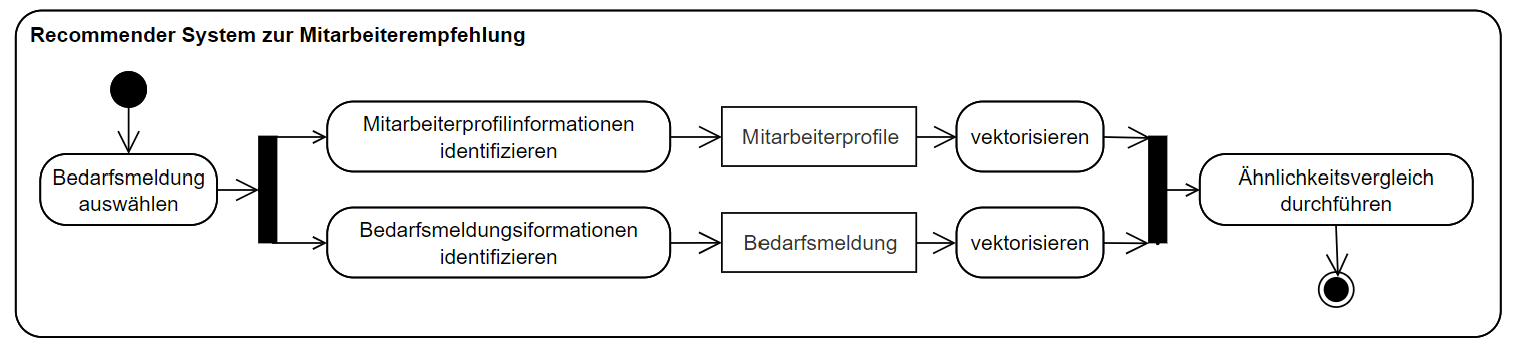
\includegraphics[width=\linewidth]{Abbildungen/recommendersystem.png}
	\caption{Abstrakte Darstellung des Recommender System zur Mitarbeiterempfehlung.}
	\label{fig:recommendersystem}
\end{figure}\mbox{} \\
Diese Schritte sind abstrakt als UML-Aktivitätsdiagramm in der Abbildung \ref{fig:recommendersystem} dargestellt. Nach Auswahl einer \emph{Bedarfsmeldung} wird diese einerseits auf die relevanten Informationen reduziert und strukturiert. Diesen Schritt gilt es in dieser Arbeit zu konzipieren, entwickeln und evaluieren. Neben diesem Schritt erfolgt eine Vorverarbeitung der Mitarbeiterprofile, bei dem die verfügbaren Informationen in eine vergleichbare Struktur wie die Bedarfsmeldung reduziert werden. Die strukturierte \emph{Bedarfsmeldung} und Mitarbeiterprofile werden vektorisiert und am Ende mit einer Vergleichsmetrik auf Ähnlichkeit geprüft. Die Komplexität der Vergleichsmetrik ist dabei skalierbar. So können verschiedene Aspekte, wie z.B. Verfügbarkeit, Skills, etc., Bestandteil des Ähnlichkeits-Scoring sein. Das Profil, bzw. die Profile mit der höchsten Ähnlichkeit zur \emph{Bedarfsmeldung} wird am Ende Empfohlen.
\paragraph{Recommender Systems Historie und aktueller Stand der Forschung}\mbox{} \\
Auch wenn die Erstellung eines vollständigen Recommender Systems nicht Gegenstand der vorliegenden Ausarbeitung ist, stellt die Nutzung von Information Retrieval und Filtering ein entscheidener Schritt in Richtung eines funktionierenden Recommender Systems dar. Das Verständnis der Funktionsweise eines Recommender Systems sowie dessen Entwicklung in den vergangenen Jahren ist daher für das Verständnis des Teilbereichs dieser Thematik von Nutzen.\\

Recommender Systems existieren bereits seit vielen Jahren \cite{dong2022brief}. Im Jahr 1992 führten Belkin und Croft eine Analyse und einen Vergleich des Information Retrievals und Filtering durch \cite{dong2022brief}. Das Information Retrieval behandelt die grundlegende Technologie der Suchmaschine \cite{dong2022brief}. Das Recommender System basiert hauptsächlich auf der Technologie des Information Filtering. Im selben Jahr präsentierte Goldberg das Tapestry-System, das das erste System zur Informationsfilterung darstellt, das auf kollaboratives Filtern durch menschliche Bewertung basiert \cite{dong2022brief}. Die Mehrheit der frühen Empfehlungsmodelle basiert auf kollaborativer Empfehlungen, wobei K-Nearest-Neighbor (KNN)-Modelle eine besondere Rolle einnehmen. Diese Modelle prognostizieren die Nachbarn eines Zielnutzers, indem sie eine Ähnlichkeit zwischen den vorherigen Präferenzen und den Präferenzen der anderen Nutzer berechnen \cite{dong2022brief}. Die Studie von Goldberg inspirierte einige Forscher des Massachusetts Institute of Technology (MIT) und der University of Minnesota (UMN) dazu, einen Nachrichtenempfehlungsdienst mit dem Namen \emph{GroupLens} zu entwickeln. Die Hauptkomponente dieses Dienstes ist ein Modell zur kollaborativen Filterung zwischen Nutzern \cite{dong2022brief}. Das gleichnamige Forschungslabor kann somit als Pionier auf dem Gebiet der Recommender Systems bezeichnet werden. Die dort durchgeführten Forschungen bilden die Grundlage für nachfolgende Musik- und Video-Ähnlichkeitsempfehlungen \cite{dong2022brief}. \\

Recommender Systeme haben in den letzten Jahren verschiedene Definitionen erhalten. Eine dieser Definitionen wird in dem Artikel von Resnick und Varian (1997) sinngemäß so beschrieben, dass ein typisches Recommender System Empfehlungen durch Personen als Eingabe erhält, die das System dann zusammenschließt und an geeignete Empfänger weiterleitet \cite{burke2011recommender}. In einigen Fällen besteht die primäre Transformation in der Zusammenführung, in anderen Fällen liegt die Fähigkeit des Systems darin, gute Übereinstimmungen zwischen Empfehlungsgebern und Empfehlungsempfängern herzustellen \cite{burke2011recommender}. Empfehlungssysteme stellen ein Instrument zur Interaktion mit umfangreichen und vielschichtigen Informationen dar. Sie ermöglichen eine personalisierte Sicht auf diese Informationen, indem sie die für den Nutzer wahrscheinlich relevanten Inhalte aufbereiten \cite{burke2011recommender}. Besonders im Handelsverkehr im Internet sind Recommender Systeme ein häufiger Einsatzgebiet. Dabei werden Recommender Systeme als Werkzeuge zum Suchen und Filtern von Informationen verwendet, die dem Benutzer Vorschläge unterbreiten, die für ihn nützlich sein könnten. Sie sind in einer Vielzahl von Internetanwendungen weit verbreitet und helfen den Nutzern, bessere Entscheidungen bei der Suche nach Nachrichten, Musik, Urlaubsangeboten oder Geldanlagen zu treffen \cite{ricci2014recommender}. Eine spezifisches Recommender System konzentriert sich normalerweise auf eine Art von Themengebiet wie z. B. Filme oder Nachrichten \cite{ricci2014recommender}. Darüber hinaus sind sie zu einem entscheidenden Faktor in der Entscheidungsfindung von Organisationen geworden \cite{chartron2014general}. Unternehmen wie \emph{adesso} bauen immer weiter auf Recommender System unterstützte System auf, um Prozesse zu beschleunigen oder zu vereinfachen. Grundsätzlich können die Methoden in die Typen (i)\emph{collaborative Filtering-based} (kollaborative Empfehlungssysteme), (ii)\emph{content-based} (inhaltsbasierte Empfehlungssysteme), (iii)\emph{knowledge-based} (wissensbasiert Empfehlungssysteme) und (iv)\emph{hybrid} (hybride Empfehlungssysteme) unterteilt werden.\\

Jede Empfehlungsmethode hat ihre Vorteile und Grenzen \cite{lu2020recommender}. Insbesondere das inhaltsbasierte Empfehlungssystem bring eine hohe Relevanz für das Mitarbeiterempfehlungssystem. Die Grundprinzipien inhaltsbasierter Empfehlungssysteme sind zum einen die Analyse der Beschreibung der von einem bestimmten Benutzer bevorzugten \emph{Items}, um die gemeinsamen Hauptattribute (Präferenzen) zu identifizieren, die diese \emph{Items} unterscheiden. Diese Präferenzen werden in einem \emph{Benutzerprofil} gespeichert \cite{lu2020recommender}. Zusätzlich werden die Eigenschaften jedes \emph{Items} mit dem \emph{Benutzerprofil} verglichen, so dass nur \emph{Items} empfohlen werden, die eine hohe Ähnlichkeit mit dem \emph{Benutzerprofil} aufweisen \cite{lu2020recommender}. Bei der Idee der Mitarbeiterempfehlung kann also die \emph{Bedarfsmeldung} mit den benötigten Projektskills und Anforderung als \emph{Benutzerprofil} angesehen werden. Die Mitarbeiterprofile sind dabei die \emph{Items}. Die Attribute werden verglichen (Skills der Mitarbeiter mit den Skills und Anforderungen der \emph{Bedarfsmeldung}) und ähnliche \emph{Items} werden vorgeschlagen. Mit Hilfe traditioneller Methoden des Information Retrievals, wie z.B. dem Kosinus-Ähnlichkeitsmaß, werden dann Empfehlungen generiert \cite{lu2020recommender}. Darüber hinaus generieren sie Empfehlungen mit Hilfe von statistischen und maschinelle Lernverfahren, die in der Lage sind, Nutzerinteressen aus historischen Nutzerdaten zu lernen \cite{lu2020recommender}.
\paragraph{Information Retrieval und Information Filtering}\mbox{} \\
%Diese Arbeit beschreibt den Unterschied zwischen Information Filtering und Information Retrieval\cite{belkin1992information}
Im Allgemeinen wird einem Informationssystem die Funktion zugeschrieben, den Benutzer zu den Dokumenten zu führen, die seinen Informationsbedarf am besten decken \cite{belkin1992information}. Allgemeiner ausgedrückt ist das Ziel eines Informationssystems, dem Benutzer Informationen aus der Wissensressource zur Verfügung zu stellen, die ihm helfen, ein Problem zu lösen \cite{belkin1992information}. Auf der anderen Seite ist unter Filtern das Entfernen von Daten aus einem eingehenden Datenstrom zu verstehen und nicht das Auffinden von Daten in diesem Datenstrom \cite{belkin1992information}. Filtersysteme verarbeiten große Datenmengen \cite{belkin1992information}. Typische Anwendungen betreffen Gigabytes von Text oder weitaus größere Mengen anderer Medien \cite{belkin1992information}. Während es bei dem Information Retrieval typischerweise um die einmalige Nutzung des Systems durch eine Person mit einem einmaligen Ziel und einer einmaligen Anfrage geht, befasst sich die Informationsfilterung mit der wiederholten Nutzung des Systems durch eine oder mehrere Personen mit langfristigen Zielen oder Interessen \cite{belkin1992information}.
\section{Anforderungsanalyse}
\label{sec:anforderungsanalyse}
Es wird eine Lösung gesucht, die eine effiziente Verarbeitung von \emph{Bedarfsmeldungen} durchführen kann. Welche Aspekte in einer \emph{Bedarfsmeldung} relevant sind, wurde bereits im Kapitel \ref{chap:erwartungshaltung} näher erläutert. Die Idee ist es, ein System zu entwickeln, die Möglichkeiten zum laden von \emph{Bedarfsmeldungen} bietet. Das System überführt die Informationen aus Jira in eine Struktur, die für die weitere Nutzung im Recommender System Kontext funktioniert. In den \emph{Bedarfsmeldungen} existieren semi strukturierte Volltexte. Diese gilt es durch Ablauf verschiedener Schritte innerhalb des System zu bearbeiten. Dabei soll der Volltext von unngewünschten Zeichen und Formatierungen befreit werden. Dadurch entsteht ein Absatz bestehend aus Wörtern. Durch die Vorverarbeitung verliert der Text an Zusammenhänge durch beispielsweise Satztrennungen durch einen Punkt. Um zusammengehörende Wörter zusammenzubringen, werden verschiedene Schritte durchlaufen. Einerseits sollen vorab Datums-Daten und Zeiten extrahiert werden, da diese durch die Vorverarbeitung durch die Entfernung von Zeichen ebenfalls entfernt werden würden. Durch eine Erstellung von Wortketten können Verbindungen zwischen zwei Wörtern untersucht werden. Eine Wortkette soll hier bedeuten, dass Wörter nebeneinanderstehende Wörter entweder verbunden oder nicht verbunden sind. Zum besseren Verständnis kann folgendes Beispiel betrachtet werden: Die drei Wörter \emph{Ich bin hier} sind durch \emph{Ich bin} und \emph{bin hier} miteinander verkettet. Würde eine Verbindung zwischen \emph{bin} und \emph{hier} getrennt werden, würden zwei Sätze entstehen, nämlich \emph{Ich bin} und \emph{hier}. Diese zusammenhänge sollen Mithilfe von zwei schritten unterbrochen werden. Einerseits sollen untypische Wortkombinationen identifiziert und entfernt werden, da diese im ursprünglichen Volltext ebenfalls nicht nebeneinander standen. Zudem sollen Wortketten ohne Schlüsselwörter herausgenommen werden, da diese dadurch nicht relevant sind. Um die Anforderungen an das System genauer zu beschreiben, wird ein Use-Case-Diagramm und ein UML-Aktivitätsdiagramm dargestellt und beschrieben. Zudem werden funktionale und nichtfunktionale Anforderungen des Systems erfasst.
\subsection{Anwendungsfälle}
\label{sec:usecase}
In diesem Kapitel werden die Interaktionen zwischen Benutzer und System beschrieben. Dazu wird ein Use-Case-Diagramm angefertigt, das eine grafische Übersicht über alle Anwendungsfälle bietet.
\begin{figure}[H]
	\centering  
	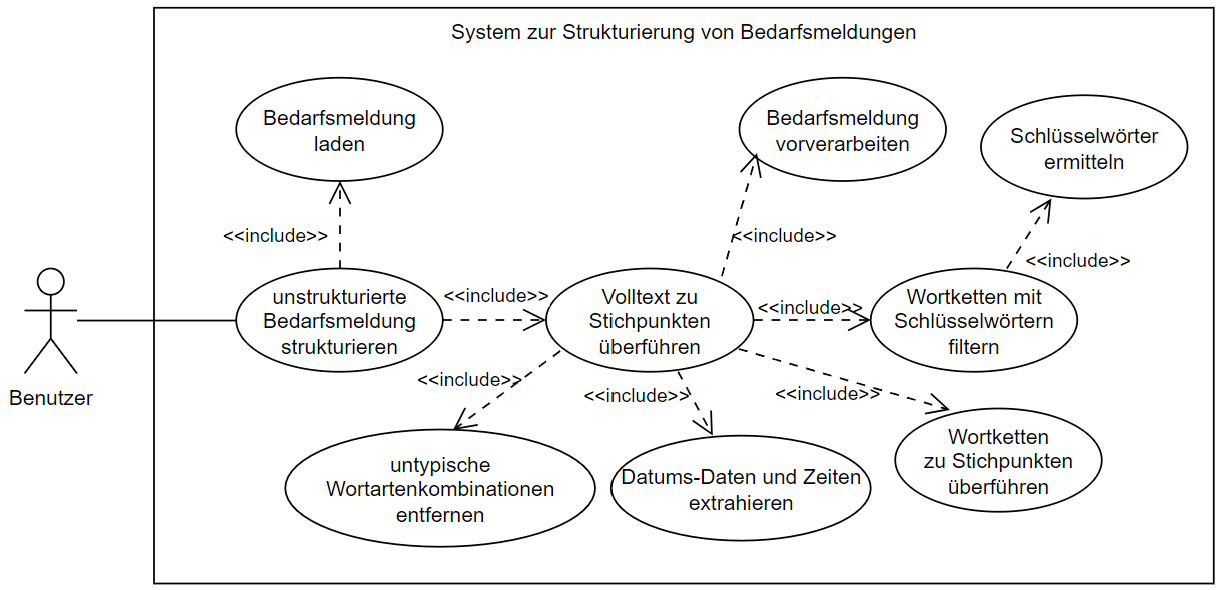
\includegraphics[width=\linewidth]{Abbildungen/use-case.png}
	\caption{Use-Case Diagramm zum System zur Strukturierung von Bedarfsmeldungen.}
	\label{fig:usecasediagrammwirklich}
\end{figure}\mbox{} \\
In der Abbildung \ref{fig:usecasediagrammwirklich} ist das Use-Case Diagramm zum System zur Strukturierung von \emph{Bedarfsmeldungen} dargestellt. Es existiert ein Akteur, der die Bezeichnung \emph{Benutzer} hat. Dieser hat die Möglichkeit unstrukturierte \emph{Bedarfsmeldungen} zu strukturieren. Dazu kann das System einerseits eine \emph{Bedarfsmeldung} laden und im Falle der unstrukturierten Volltexfelder eine Reihe an Aufgaben durchführen. Um die Volltexte in Stichpunkte zu überführen, kann der Text mit Vorverarbeitungsverfahren reduziert und angepasst werden. Im Rahmen der Überführung von Stichpunkten können die aus den Volltext erstellten Wortketten auf die gekürzt werden, die mindestens ein Schlüsselwort enthalten. Die Schlüsselwörter können zudem ermittelt werden. Im Anwendungsfall der Überführung des Volltextes in Stichpunkte, können Wortartkombinationen, die nicht zusammengehören in den Wortketten entfernt werden. Dadurch trennen sich neben der Filterung von Schlüsselwörter weitere Verbindungen innerhalb der Wortketten. Datums- und Zeitangaben können neben den anderen Anwendungsfällen separat herausgefiltert werden. Schließlich können die Wortketten zu Stichpunkten überführt werden.
%Dieser hat die Möglichkeit eine oder mehrere \emph{Bedarfsmeldungen} zu laden. Zudem kann diese ins Englische übersetzt werden. Darüber hinaus kann die \emph{Bedarfsmeldung} durch \emph{Preprocessing} vorverarbeitet werden und irrelevante Wörter und Zeichen aus der \emph{Bedarfsmeldung} ausschließen. Der Benutzer kann die Methoden \emph{TF-IDF}, \emph{TextRank}, \emph{N-Gram}, \emph{POS-Tagging} und \emph{NER} mit der \emph{Bedarfsmeldung} anwenden. Wenn mehrere Methoden in der Pipeline sind, können die Resultate durch die Anwendung von \emph{Data-Fusion} zusammengeführt werden.
\subsection{Anforderungen}
Im Folgenden werden die funktionalen sowie nichtfunktionalen Anforderungen des Systems beschrieben. Diese Informationen wurden aus den Ergebnissen des Kapitels \ref{chap:erwartungshaltung} und dem Kapitel \ref{sec:anforderungsanalyse} hergeleitet und bilden den Rahmen des Systems.
\subsubsection{Funktionale Anforderungen}
Die funktionalen Anforderungen beschreiben konkrete Funktionalitäten des Systems. Dazu werden zusammengehörende Anforderungen nummeriert und in detaillierte Unterpunkte aufgelistet und beschrieben.
\begin{enumerate}[label=1.\arabic*]
	\item Die \emph{Bedarfsmeldungen} sollen geladen werden können.
	\item Beim laden wird eine \emph{Bedarfsmeldung} ausgewählt.
	\item Die ausgewählte \emph{Bedarfsmeldung} muss in die vordefinierte Struktur überführt werden.
\end{enumerate}
\begin{enumerate}[label=2.\arabic*]
	\item Das System soll Methoden der Vorverarbeitung zur Bereinigung eines Volltextes anwenden können.
	\item Die Vorverarbeitung soll ein Volltext als Eingabe erhalten.
	\item Das Vorverarbeitung soll den bereinigten Volltext als Ausgabe zurückgeben.
\end{enumerate}
\begin{enumerate}[label=3.\arabic*]
	\item Das System soll eine Methode zur Identifizierung von Schlüsselwörtern anwenden können.
	\item Das Modul soll eine Liste mit Schlüsselwörtern anlegen.
\end{enumerate}
\begin{enumerate}[label=4.\arabic*]
	\item Das System soll Wortketten aus einem Volltext erstellen können.
	\item Das Modul soll einen Volltext als Eingabe für diese Methode erhalten.
	\item Als Rückgabe soll das Modul eine Liste mit Wortketten zurückgeben.
	\item Das System soll eine Wortketten-Liste auf die Wörter reduzieren, die mindestens ein Schlüsselwort enthalten.
\end{enumerate}
\begin{enumerate}[label=5.\arabic*]
	\item Das System soll eine Methode zur Extraktion von Zeitangaben anwenden können.
	\item Das Modul soll aus einem Volltext Datums- und Zeitangaben extrahieren.
\end{enumerate}
\begin{enumerate}[label=6.\arabic*]
	\item Das System soll eine Methode zur Identifikation von untypischenn Wortkombinationen anwenden können.
	\item Das Modul soll Wortkombinationen aus der Wortkette erhalten und überprüfen ob die Wörter nebeneinander stehen dürfen.
	\item Wortketten werden entfernt, die nicht nebeneinander stehen sollen.
\end{enumerate}
\begin{enumerate}[label=7.\arabic*]
	\item Das System soll die Wortketten in zusammengehörende Stichpunkte zusammenführen.
	\item Als Ergebnis wird eine Liste mit Stichpunkten zurückgegeben.
\end{enumerate}
\begin{enumerate}[label=8.\arabic*]
	\item Die in Stichpunkte umgebauten Volltexte werden der \emph{Bedarfsmeldung} beigefügt.
	\item Die Datums- und Zeitangaben werden den Stichpunkten beigefügt.
	\item Das Ergebnis wird dem Benutzer ausgegeben.
\end{enumerate}
\subsubsection{Nichtfunktionale Anforderungen}
Hierbei handelt es sich um qualitätsbezogene Anforderungen. Diese umfassen nicht konkrete Funktionen des Systems, sondern stellen Rahmenbedingungen des Systems im Ganzen zusammen.
\begin{enumerate}
	\item Das System soll modular aufgebaut sein, um die einzelnen Schritte und Methoden austauschen zu können.
	\item Das System soll in der Lage sein, mehrere \emph{Bedarfsmeldungen} laden zu können.
	\item Das System muss in der Lage sein, die \emph{Bedarfsmeldungen} in einer akzeptablen Zeitspanne zu verarbeiten.
	\item Das Ergebnis muss deterministisch sein.
\end{enumerate}
\subsection{Ablauf des Systems}
Der Ablauf des Systems zur Strukturierung von \emph{Bedarfsmeldungen} wird mit Hilfe eines UML-Aktivitätsdiagramm dargestellt, das eine Erweiterung des Aktivitätsdiagramms aus der Abbildung \ref{fig:recommendersystem} durch eine Hierarchische Schachtelung darstellt.
\begin{figure}[H]
	\centering  
	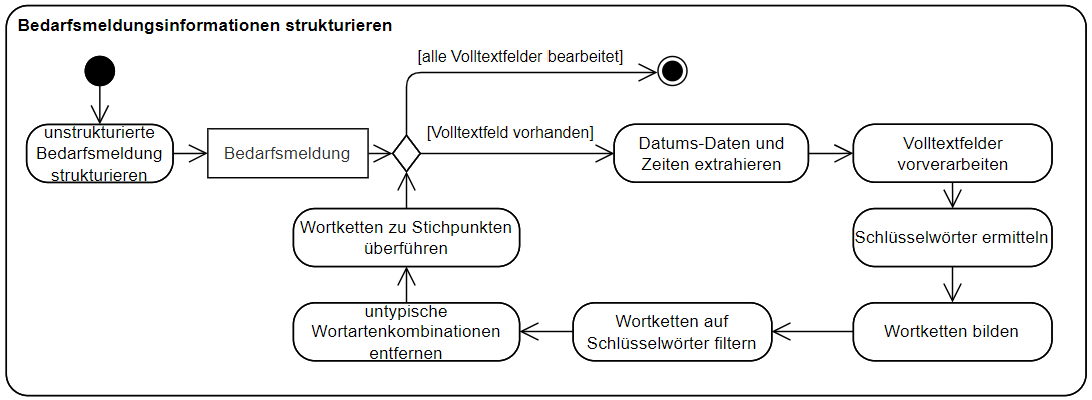
\includegraphics[width=\linewidth]{Abbildungen/bedarfsmeldungstrukturieren.png}
	\caption{Abstrakte Darstellung des Systems zur Strukturierung von \emph{Bedarfsmeldungen}.}
	\label{fig:ablaufsystemabstrakt}
\end{figure}\mbox{} \\
In Abbildung \ref{fig:ablaufsystemabstrakt} ist der abstrakte Ablauf des Systems dargestellt. Zu Beginn wird der unstrukturierte Informationsfelder mit \emph{Bedarfsmeldungsinformationen} in eine strukturierte Form gebracht. Anschließend werden die Volltextfelder durch eine Reihe an Schritten geleitet. Angefangen mit der Extraktion von Datums-Daten und Zeiten. Die Volltextfelder werden vorverarbeitet, wodurch ungewollte Formatierungen entfernt werden. Darauffolgend werden Schlüsselwörter im Volltext ermittelt. Aus dem Volltext werden Wortketten gebildet und auf die Wörter reduziert, die Schlüsselwörter enthalten. Dann werden untypische Wortartenkombinationen entfernt, wodurch die Wortketten weiter separiert werden. Zum Schluss werden die einzelnen Wortketten in Stichpunkte überführt und in die \emph{Bedarfsmeldung} aufgenommen. Dieser Prozess wird für alle Volltextfelder durchgeführt.

\chapter{Literaturüberblick}
\label{chap:literaturüberblick}

\section{Verwandte Arbeiten}
%\label{sec:forschung-und-ansätze}

-Einschätzen der Fähigkeiten, Talente und des Fachwissens der Mitarbeiter\\
-In diesem Papier wird ein Ansatz beschrieben, um aus Unternehmensdaten und den digitalen Fußabdrücken der Mitarbeiter Informationen zu gewinnen.\\
-Beurteilung des Fachwissens eines Mitarbeiters in einem breiten Bereich wie cloud computing oder cybersecurity\\
-Auf einer hohen Ebene lässt sich der Ansatz der Informationsbeschaffung und -fusion wie folgt beschreiben: Es wird eine Liste von Suchbegriffen erstellt, die sich auf das breite Fachgebiet beziehen.\\
-Die Suche wird nach jedem dieser Abfragebegriffe durchgeführt, um Beweise für Mitarbeiter und Datenquellen zu finden. Die verschiedenen Beweisstücke werden miteinander verschmolzen, gewichtet und nach der Abfrage sortiert. Die Mitarbeiter werden nach Datenquelle gewichtet und möglicherweise auf andere Weise bewertet, um einen einzigen Ordinalwert (sehr niedrig, niedrig, moderat, etwas, begrenzt) für ihr Fachwissen in diesem breiten Bereich zu erhalten.\cite{horesh2016information} \\

information filtering\\
-Informationen für seine Benutzer betreffend der Anwender in Bezug auf ihre Interessengebiete zu reduzieren
-Dazu werden nicht relevante Dokumente aus einem Strom von Informationen entfernt, sodass den Anwendern nur relevante Dokumente präsentiert werden.
-Ein Teil der Arbeit beschäftigt sich mit der der Informationsfilterung und mögliche Filterungsvarianten werden vorgestellt. Die Arbeit konzentriert sich auf die inhaltsbasierte Filterung von Textdokumenten und identifizieren Informationsfilterung als einen Spezialfall der Textklassifikation.
-Überblick über gängige Methoden. Anschließend werden bekannte Filterungsprojekte kurz vorgestellt, bevor verwandte Aufgaben verglichen werden.
\cite{lanquillon2001enhancing}

preprocessing
\cite{alasadi2017review}
-Wege und Schritte zur Aufbereitung von Datensätzen
-Arbeit umfasst Data-Mining Vorverarbeitung um Qualität der Daten zu verbessern
-Wichtiger Schritt um Effizienz zu verbessern

-------
spam-filter\\
-Überblick über verfügbare Methoden, Herausforderungen und zukünftige Forschungsrichtungen im Bereich der Spam-Erkennung, Filterung und Eindämmung von SMS-Spam. Dabei werden auch Methodiken der keyword frequency ratio und Herunterbrechung auf keyword components behandelt \cite{shafi2017review}\\

----
In diesem Beitrag werden Studien zu Technologien vorgestellt, die für die Suche und das Abrufen von Informationen im Web nützlich sind. Es wird aufgezeigt, dass Information Retrieval und Ranking im Web-Kontext anders Funktioniert als in einer statischen Datenbank. \cite{kobayashi2000information}\\

Die Kombination von verschiedenen Textdarstellungen und Suchstrategien ist zu einer Standardtechnik geworden, um die Effektivität der Informationsbeschaffung zu verbessern.\cite{croft2000combining}\\

In dieser Arbeit wird eine Pipeline entwickelt, die die N-Gramm-Analyse verwendet, um Schlagwörter aus einem Text zu extrahieren und mit verschiedenen Ansätzen von Word-Clouds zu visualisieren.\cite{pirk2019implementierung}\\

python pipeline mit python und tf-idf. Beschreibt warum TF-IDF häufig in  als Vorverarbeitung beim maschinellen Lernen eingesetzt wird. Hat in der Regel einen höheren Vorhersagewert als rohe Termhäufigkeit. Die Gewichtung von Themenwörtern wird erhöt,, um die Bedeutung von Wörtern zu erhöhen, während die Gewichtung von hochfrequenten Funktionswörtern verringert wird.\cite{lavin2019analyzing}\\

Kombination drei Ansätze Ansätze. Unter anderem auch TF-IDF. Kombinieren mit einem sogenannten CLASSIFIER Model. Das Klassifikationsmodell bezieht sich direkt auf die
Ergebnisse der Modelle LSTM, VADER und TFIDF, die jeweils drei Eingaben liefern. Die Werte dieser Eingaben liegen im
Bereich von [0,1].
Die Ausgabe des Klassifikationsmodells ist binär und liefert eine Vorhersage der
Stimmung des vollständigen Textes der Modelleingabe (positiv oder negativ).\cite{chiny2021lstm}\\

Das erste vorverarbeitete Dokument wird mithilfe eines Extraktionsalgorithmus
analysiert und anschließend wird für jeden Begriff TF/IDF berechnet.
Danach werden alle TF/IDF-Begriffe für jeden Satz summiert.
Im nächsten Schritt werden alle Sätze anhand der Summe von TF/IDF eingestuft.
Das Kompressionsverhältnis bestimmt die Position des Satzrangs. In dieser Studie wird eine Kompression von 50\% verwendet, was bedeutet,
dass die Satzzusammenfassung um 50\% des Originaltextes gekürzt wird. Nach der Auswahl des Satzes wird seine Berechnung durchgeführt.
Ähnlichkeit wird mit der Cosinus-Ähnlichkeitsmethode berechnet. 
Anschließend werden alle Sätze anhand ihrer Cosinus-Ähnlichkeit von der höchsten zur niedrigsten sortiert.
Der resultierende Text mit
neuer Satzanordnung ist die endgültige Zusammenfassung.\cite{darmawan2015hybrid}\\


Kombination aus TD-IDF und N-Gram. Um Fake news heraus zu filtern\cite{suhasini2021hybrid}

Named ENtity Recognition mit POS-Tagger Implementierung mit Spacy für die griechische Sprache\cite{partalidou2019design}\\

Preprocessing von Softwareanforderungen. Generierung aus Text Anforderungen zu diversen Diagrammen etc \cite{kroha2000preprocessing}

\newpage
g
\newpage
g
\newpage
g
\newpage
g
\newpage
g
\newpage
g
\newpage

\section{Definitionen und Konzepte: Information Retrieval, Data-Mining, Bedarfsmeldungen}
\label{sec:definitionen-konzepte}

Diese Arbeit beschreibt den Unterschied zwischen Information Filtering und Information Retrieval\cite{belkin1992information}

%\section{Relevante Methoden und Techniken im Bereich Information Retrieval und Data-Mining}
%\label{sec:relevante-methoden}
\newpage
g
\newpage
g
\newpage







\chapter{Umsetzung}
\label{chap:implementierung}
Auf Basis welcher Methodiken und Ansätze die relevanten Informationen extrahiert werden können, wurde in Kapitel \ref{sec:literaturueberblick} dargestellt. Nun gilt es diese Ansätze in einem System zu implementiert. In diesem Kapitel werden die Funktionalitäten der Pipeline zusammengetragen. Dabei werden verwendete Technologien und Implementationsaspekte genauer beschrieben.
\section{Beschreibung}
Damit alle Ansätze und Methoden zur Extraktion von Informationen gut funktionieren und vergleichbar bleiben, wird eine Übersetzungsfunktion der \emph{Bedarfsmeldungen} hinzugefügt. Auch wenn die \emph{Bedarfsmeldungen} in den meisten Fällen auf Deutsch sind, hilf es diese zu übersetzen, damit keine Unterschiede in der Ergebnisqualität resultiert, da einige Methoden und Ansätze auf Basis von Englischen Trainingssätzen trainiert wurden. Schließlich müssen alle aus Kapitel \ref{sec:literaturueberblick} untersuchten Ansätze implementiert und nutzbar sein. Sie sollen die Möglichkeit haben \emph{Bedarfsmeldungen} als Input zu erhalten und eine strukturierte \emph{Bedarfsmeldung} als Ausgabe zurückzugeben. Zur vereinfachten Entwicklung soll das System modular sein, damit Methoden und Ansätze nach belieben durchgetauscht und verwendet werden können.\\
\section{Konkreter Ablauf der Pipeline}
Dieses Kapitel beschreibt den Ablauf der Pipeline. Dazu wird das Aktivitätsdiagramm aus der Abbildung \ref{fig:ablaufsystemabstrakt} verfeinert und mit allen analysierten Komponenten aus Kapitel \ref{sec:literaturueberblick} genauer beschrieben.
\begin{figure}[H]
	\centering  
	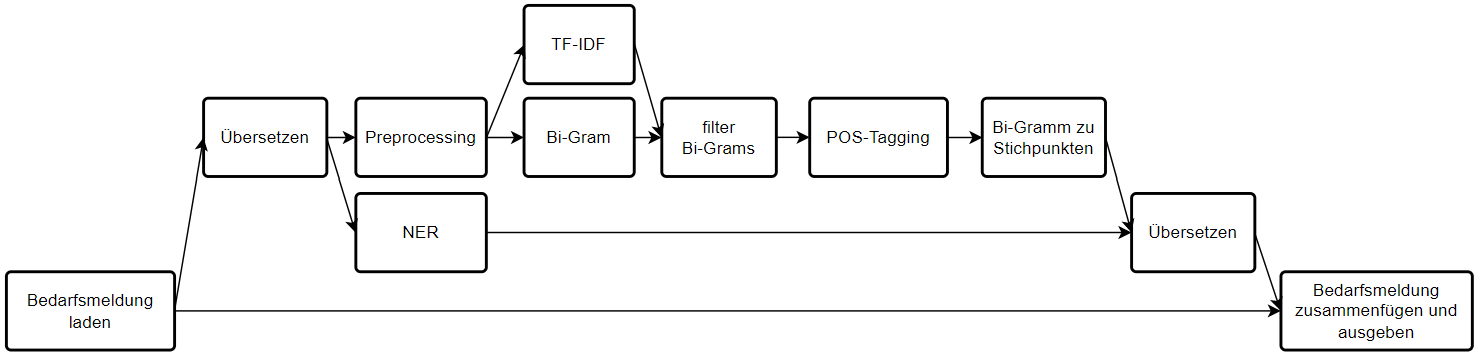
\includegraphics[width=\linewidth]{Abbildungen/flowchart.png}
	\caption{Flussdiagramm der Pipeline.}
	\label{fig:flowchart}
\end{figure}\mbox{} \\
Die Abbildung \ref{fig:flowchart} zeigt das UML-Aktivitätsdiagramm der Python Pipeline zur Strukturierung von \emph{Bedarfsmeldungen}. Im ersten Schritt \emph{unstrukturierte Bedarfsmeldung strukturieren} im Ablauf der Pipeline wird eine \emph{Bedarfsmeldung} ausgewählt und in die festgelegte \emph{Bedarfsmeldungsstruktur} aus Kapitel \ref{sec:strukturierungbedarfsmeldung} umgebaut. Die Felder \emph{Einsatzbeginn} und \emph{Einsatzende} werden zu einem Feld \emph{Einsatz} zusammengefügt. Neben den Feldern \emph{Aufgaben} und \emph{Skills} bleiben alle weiteren Felder bis zum letzten Punkt Ausgabe unverändert. Die Felder \emph{Aufgaben} und \emph{Skills} werden jeweils in die Schleife weitergeleitet, wo sie auf Stichpunkte reduziert werden. Der Prozess zur Reduktion durchläuft mehrere Schritte. Zu Beginn werden die Volltexte aus den Feldern im Punkt \emph{ins Englische übersetzen} übersetzt. Anschließend erfolgt im Schritt \emph{Datums-Daten und Zeiten mit NER extrahieren} zum einen die Extrahierung der zeitbezogenen Daten. Darauffolgend wird der Volltext im Punkt \emph{Preprocessing} für die weitere Nutzung vorverarbeitet. Der Grund warum die Extraktion mit \emph{NER} nicht nach der Vorverarbeitung durchgeführt werden kann ist, da im Vorverarbeitungsschritt alle Nummern und somit auch alle zeitbezogenen Daten entfernt werden. Die Resultate des \emph{NER} werden zum Ende hin zurück ins deutsche übersetzt und der fertigen Stichpunktliste beigefügt. Zur Erstellung der Stichpunktliste werden relevante Schlüsselwörter durch die \emph{TF-IDF}-Methode ermittelt. Anschließend wird der vorverarbeitete Text zu \emph{Bi-Grammen} umgeformt. Beim Punkt \emph{Bi-Gramme auf Schlüsselwörter filtern} werden alle \emph{Bi-Gramme} entfernt, die kein Schlüsselwort aus der \emph{TF-IDF}-Methode enthalten. Somit erhält der Schritt \emph{untypische Wortartenkombinationen mit POS-Tagging entfernen} eine reduzierte Liste mit \emph{Bi-Grammen}, bei dem mindestens eines der beiden \emph{Bi-Gramm}-Wörter ein Schlüsselwort Wort darstellt. Jedes Wort der \emph{Bi-Gramm}-Liste durchläuft eine weitere Filterung. Im Englischen existieren Wortarten, die typischerweise nicht nebeneinander stehen. Durch Entfernung dieser \emph{Bi-Gramme} durch POS-Tagging-Kombinationen erfolgt eine weitere Trennung der Wortketten in der \emph{Bi-Gramm}-Liste. Wörter die nicht zusammengehören, verlieren dadurch die Verbindung zueinander. Im darauf folgenden Schritt \emph{Bi-Gramm zu Stichpunkten überführen} werden die \emph{Bi-Gramme} jeweils zu einem String zusammengefügt, bei dem im darauf Folgendem \emph{Bi-Gramm} ebenfalls ein relevantes Wort enthalten sind. Dadurch formt sich eine Liste mit Stichpunkten bestehend aus eins bis x vielen Wörtern, die Bezug zueinander haben. Im Schritt \emph{ins Deutsche übersetzen} wird die Liste mit Stichpunkten zurück ins übersetzt. Dieser Ablauf wird für die beiden Felder \emph{Aufgaben} und \emph{Skills} durchlaufen, da diese Volltextfelder darstellen.
\section{Implementationsdetails}
Dieses Kapitel beschreibt den technischen Entwicklungsprozess zur Umsetzung der Anforderungen des Systems. Die Implementierung fokussiert sich auf die Umsetzungen von Technologien und Funktionsweisen verschiedener Anforderungen. Zudem wird die Struktur des Projektes aufgezeigt.
\subsection{Pipeline}
Die Pipeline wurde in der Programmiersprache Python umgesetzt. Python hat sich zu einer der populärsten interpretierten Programmiersprachen entwickelt \cite{mckinney2012python}. Die Programmiersprache eignet sich insbesondere für die Erstellung kleiner Programme und Skripte, die zur Automatisierung von Aufgaben eingesetzt werden können \cite{mckinney2012python}. Python hat eine große und aktive Community für wissenschaftliche Berechnungen und Datenanalysen hervorgebracht und hat sich in den letzten Jahren zu einer der wichtigsten Sprachen für Data Science, maschinelles Lernen und allgemeine Softwareentwicklung in Wissenschaft und Industrie entwickelt \cite{mckinney2012python}. Python unterstützt Modularität, wodurch ein Teil der Anforderungen somit abgedeckt werden kann. Die Implementierungen der einzelnen Verfahren aus den Anforderungen werden nicht manuell, sondern auf Basis von bereits existierende Bibliotheken umgesetzt.
\subsection{Projektstruktur}
\label{sec:projektstruktur}
Das Projekt wird in einem git Repository gespeichert und versioniert. Die Projektstruktur ist ohne zusätzliche Konfigurationsdateien wie folgt aufgebaut:
\dirtree{%
	.1 .git/.
	.2 modules/.
	.3 ner.py.
	.3 nGram.py.
	.3 posTagging.py.
	.3 preprocessing.py.
	.3 readRequirements.py.
	.3 textRankingAlgorithm.py.
	.3 tfIdf.py.
	.3 transformRequirements.py.
	.3 translate.py.
	.2 requirements/.
	.3 jiraTickets.json.
	.3 preprocessedRequirements.json.
	.3 ....
	.2 app.py.
	.2 ....
}
Die einzelnen Module aus dem Flussdiagramm in Kapitel \ref{fig:flowchart} sind im Verzeichnis \url{modules/} in separaten \url{.py} Dateien gelagert. Die \emph{Bedarfsmeldungen} werden im \url{requirements/}-Verzeichnis gespeichert. Alle relevanten \emph{Bedarfsmeldungen} sind in der \url{jiraTickets.json}-Datei in einer Liste gespeichert. Die Datei \url{app.py} ist der Kern der Pipeline. Diese importiert alle Module und implementiert die Struktur der Pipeline. Das Projekt kann über den Befehl \lstinline{> py app.py} ausgeführt werden.
\subsection{Modulimplementationen}
Nachfolgend werden Implementationsdetails zu den einzelnen Modulen gegeben. Dabei werden verwendete Bibliotheken und Code-Details näher erläutert.
\paragraph{Strukturierung von Bedarfsmeldungen}\mbox{}\\
Die \emph{Bedarfsmeldungen} wurden über die Jira-Schnittstelle extrahiert und im Verzeichnis \url{requirements/jiraTickets.json} gespeichert. Zur Eingrenzung der Datenmenge wurde ein Filter angewendet, der nur die \emph{offenen} und \emph{eskalierten} \emph{Bedarfsmeldungen} zurückgibt. Diese sind die relevanten und noch aktuellen \emph{Bedarfsmeldungen}. Zudem wurden alle unrelevanten Felder mit einem weiteren Filter herausgenommen. Die Daten aus der Jira-API bestehen namentlich aus \emph{customfields} mit einer angehangenden ID. Der Softwareprototyp lädt in dem Modul \emph{readRequirements.py} die unstrukturierten Fields und formt diese in dem Modul \emph{transformRequirements.py} in \emph{Bedarfsmeldungs}-Objekte um.
\begin{center}
	\begin{tabularx}{1\textwidth} { 
			| >{\raggedright\arraybackslash}X 
			| >{\raggedright\arraybackslash}X
			| >{\raggedright\arraybackslash}X | }
		\hline
		Display-Felder & Jira-API-Felder & Objekt-Felder \\
		\hline
		\hline
		Überschrift & summary & header\\
		\hline
		Rolle & customfield\_15321 & role\\
		\hline
		Aufgaben & customfield\_10288 & tasks\\
		\hline
		Skills & customfield\_10296 & skills\\
		\hline
		Skill-Level & customfield\_15322 & skillLevel\\
		\hline
		Kunde & customfield\_10279 & customer\\
		\hline
		Einsatzort & customfield\_10297 & location\\
		\hline
		Beginn & customfield\_10293 & timePeriod\\
		\hline
		Ende & customfield\_10294 & timePeriod\\
		\hline
		Tagessatz & customfield\_10298 & dailyRate\\
		\hline
	\end{tabularx}\\
	\captionof{table}{Übersicht der Datenfelder}
	\label{tab:jiradaten}
\end{center}
In der Tabelle \ref{tab:jiradaten} ist in der ersten Spalte eine Übersicht der Datenfelder, wie diese in der Abbildung \ref{fig:jiraafter} mit dem Mockup einer standardisierten \emph{Bedarfsmeldung} auftauchen. In der zweiten Spalte sind die dazugehörigen Feldernamen, die in der \url{jiraTickets.json} enthalten sind. Die dritte Spalte spiegelt die jeweiligen Namen innherhalb des  \emph{Bedarfsmeldungs}-Objekts im Prototypen wieder. Das  \emph{Bedarfsmeldungs}-Objekt dient der strukturierten Handhabung der \emph{Bedarfsmeldungs}-Daten innerhalb des Systems.

%Um einen Freitext aus einer einzelnen \emph{Bedarfsmeldung} für die Pipeline zu laden werden Daten mit der Endung \url{.txt} verwendet.
%\begin{lstlisting}[caption={Implementation der Methode read() des Moduls \emph{readRequirements.py}}, label=lst:read]
%	def read(filename):
%		path = os.path.join(PATH, filename)
%		file = open(path, "r", encoding="utf-8")
%		content = file.read()
%		file.close()
%		return content
%\end{lstlisting}
%Im Listing \ref{lst:read} ist die Implementierung der Methode zum laden eines Freitextes dargestellt. Durch ein mitgelieferten Parameter \emph{filename} wird der Name der Datei in Zeile 2 an den Pfad angehängt. Mit der Methode \lstinline{open()}
%aus Zeile 3 kann die Datei geladen werden. Die Methode erhält die Parameter Pfad, \emph{'r'} (read) und das encoding \emph{'utf-8'}. Das encoding ist dabei Entscheidend, damit die unstrukturierten \emph{Bedarfsmeldungen} laden können. Bei der Pflege in Jira wird wenig Wert auf eine einheitliche Struktur. Somit können Zeichen enthalten sein, die beim öffnen nicht erkannt werden und eine Fehlermeldung wird zurückgegeben. Zur Vermeidung dieses Fehlers wird das encoding festgelegt. Nach dem laden durch die Methode \lstinline{read()} wird der Inhalt der \url{.txt} Datei in der Variable \emph{content} gespeichert und zurückgegeben.
\paragraph{Übersetzung}\mbox{}\\
Das Modul \emph{translate.py} ist dazu da, um die \emph{Bedarfsmeldungen} zu übersetzen. Für die Übersetzung wurde die Python Bibliothek \emph{deep-translator} verwendet. Diese bietet Implementationen unterschiedlicher Übersetzungs-APIs von diversen Anbietern. Der Vorteil ist dabei die vereinfachte Möglichkeit Anbieter bei Bedarf zu wechseln.
%\begin{lstlisting}[caption={Implementation des Moduls \emph{translate.py}}, label=lst:translate]
%	from deep_translator import GoogleTranslator
%	
%	def translate(text):
%		translated = GoogleTranslator(source='auto', target='en').translate(text)
%		return translated
%\end{lstlisting}
%Das Listing \ref{lst:translate} zeigt die Implementation des Moduls. 
Es wurde sich für den Google Translator entschieden, da hierfür kein API-Key benötigt wird. Die Methode erhält einen Text als Parameter. Der Google Translator erhält die Parameter \emph{source} und \emph{target}, beidem \emph{source} angibt in welcher Sprache der Eingabetext ist. Durch Angabe von \emph{'auto'} wird die Sprache ermittelt. Der Grund dafür ist, dass grundsätzlich anderssprachige \emph{Bedarfsmeldung} enthalten sein können. Der Parameter \emph{target} ist die Zielsprache in welche der Input übersetzt werden soll. Die Zielsprache ist hier Englisch (\emph{'en'}).
\paragraph{NER}\mbox{}\\
Um die Methode \emph{NER} zu Implementieren wurde die Bibliothek \emph{spaCy} und das Modell \emph{en\_core\_web\_sm} verwendet. 
%\begin{lstlisting}[caption={Implementation des Moduls \emph{ner.py}}, label=lst:ner]
%	import spacy
%	nlp = spacy.load("en_core_web_sm")
%	ner_categories = ["ORG","FAC","GPE","PRODUCT", "EVENT", "LANGUAGE", "DATE", "QUANTITY"]
%	def useNER(requirement):
%		tokenized = nlp(requirement)
%		entities = []
%		for ent in tokenized.ents:
%			if ent.label_ in ner_categories:
%				entities.append((ent.text, ent.label_))
%	return entities
%\end{lstlisting}
Die zu extrahierende Kategorie ist Datum (DATE). Innerhalb der Methode \lstinline{useNER()} wird der Volltext als Parameter übergeben und zu Tokens umgeformt. Anschließend werden alle Tokens durchlaufen und nach ihren Kategorien überprüft. Ist ein Token die definierte Kategorie, wird der Token in eine separate Liste gespeichert und zurückgegeben. Die extrahierten Tokens werden aus dem Volltext entfernt, um am ende keine doppelten Stichpunkte zu erhalten.
\paragraph{Preprocessing}\mbox{}\\
Vor der weiteren Nutzung der Daten innerhalb einer \emph{Bedarfsmeldung}, ist es erforderlich diese von irrelevanten Wörtern, Zeichen und Formatierungen zu befreien.% Zur Entfernung von Satzzeichen wurde die Bibliothek \emph{string} verwendet.
%\begin{lstlisting}[caption={Implementation der Methode removePunctuation() des Moduls \emph{preprocessing.py}}, label=lst:punctuation]
%	import string
%	def removePunctuation(text):
%		content=""
%		for i in text: 
%			if i not in string.punctuation:
%				content+=i    
%		return content
%\end{lstlisting}
%Im Listing \ref{lst:punctuation} ist die Implementierung dargestellt. Die \emph{Bedarfsmeldung} wird in Zeile 2 als Parameter übergeben. In Zeile 4 erfolgt ein Durchlauf jedes Zeichens innerhalb der \emph{Bedarfsmeldung}. Falls innerhalb der Schleife das Aktuelle Zeichen kein Satzzeichen enthält wird dieses in die Variable \emph{content} zwischengespeichert. Nach Abschluss der Schleife wird die Variable zurückgegeben. 
Zur Eliminierung wiederaufgetretener Wörter, die keine Relevanz für den Informationsgehalt aufweisen, wurde die Bibliothek \emph{nltk} verwendet. Diese beinhaltet eine Liste an sogenannten \emph{stopwords}.
%\begin{lstlisting}[caption={Implementation der Methode removeStopwords() des Moduls \emph{preprocessing.py}}, label=lst:stopwords]
%	from nltk.corpus import stopwords
%	def removeStopwords(text):
%		words=[word for word in text.split(" ") if word not in set(stopwords.words('english'))]
%		return " ".join(str(word) for word in words)
%\end{lstlisting}
%Im Listing \ref{lst:stopwords} ist die Implementierung zur Entfernung von \emph{stopwords} dargestellt. In Zeile 3 
Es werden alle mit einem Leerzeichen getrennten Wörter aus der übergebenen \emph{Bedarfsmeldung} in einer Liste aufgeteilt. Dabei wird jeder Listeneintrag mit der \emph{stopword}-Liste von \emph{nltk} verglichen. Stimmt das Wort nicht mit einem Eintrag der \emph{stopwords} überein, wird diese in die Liste \emph{words} hinzugefügt. Zum Schluss werden die Wörter wieder zu einem String zusammengetragen und zurückgegeben. \\

Um weitere Formatierungen und ungewünschte Zeichen zu entfernen wird die Bibliothek \emph{re} verwendet. Diese kann Regular Expression-Patterns anwenden und Bereiche, die zum Pattern passen entfernen.
%\begin{lstlisting}[caption={Implementation der Methode removeTags() und removeSpecialCharactersAndDigits() des Moduls \emph{preprocessing.py}}, label=lst:re]
%	import re
%	def removeTags(text):
%		return re.sub("</?.*?>"," <> ",text)
%	
%	def removeSpecialCharactersAndDigits(text):
%		return re.sub("(\\d|\\W)+"," ",text)
%\end{lstlisting}
%Im Listing \ref{lst:re} sind Implementationsdetails zur Entfernung von Tags und ungewollte Zeichen dargestellt. 
Die Methode \lstinline{removeTags()} erhält die Expression \lstinline{</?.*?>}. Dabei werden \lstinline{<Tags>} ermittelt und mit der Methode \lstinline{sub()} entfernt. Zur Entfernung von Ziffern und Nicht-Alphanummerischen Zeichen wird die Expression \lstinline{(\\d|\\W)+} angewendet. Als Ergebnis des Preprocessing wird ein gesäuberter String ohne Zeichen und Tags zurückgegeben. Zum schluss werden alle Wörter in Kleinbuchstaben umgewandelt. Der Grund dafür ist, dass somit die Vergleichbarkeit der Wörter gefördert wird. Es könnte sonst vorkommen, dass Beispielsweise beim Schlüsselwörterabgleich zwei Wörter nicht als identisch identifiziert werden, da sie einmal mit großem und eimal mit kleinem Anfangsbuchstaben geschrieben wurde.
\paragraph{TF-IDF}\mbox{}\\
Vorbereitend für die \emph{TF-IDF}-Methode wurden die \emph{Skills} und \emph{Aufgaben} aus allen \emph{Bedarfsmeldungen} ins Englische übersetzt, Preprocessed und in einem String zusammengefasst. Der Grund dafür ist, dass für die \emph{TF-IDF}-Methode ein Textkorpus benötigt wird, woraus die Schlüsselwörter durch \emph{Term Frequency} ermittelt werden. Damit dieser Prozess nur einmal erfolgen muss, wurden die Ergebnisse in die \url{requirements/preprocessedRequirements.json} gespeichert. Für die Implementierung des \emph{TF-IDF} wurden die Bibliotheken \emph{sklearn} und \emph{numpy} verwendet. Der Textkorpus wird dem \emph{TfidfVectorizer} von \emph{sklearn} beigefügt und die \emph{TF-IDF}-Werte werden berechnet. Anschließend werden alle durchschnittlichen \emph{TF-IDF}-Werte für jedes Wort im gesamten Textkorpus berechnet. Daraus wird eine Liste mit Wörtern und ihren durchschnittlichen \emph{TF-IDF}-Werten erstellt und in absteigender Reihenfolge sortiert. Durch ein vordefinierten Score Threshold können darunterliegende Schlüsselwörter entfernt werden. Dies ist wichtig, damit Wörter mit niedrigem Scoring und diese Beispielsweise nur einmal im Textkorpus auftauchen nicht als Schlüsselwörter erfasst werden. Als Ergebnis wird eine Liste mit Schlüsselwörtern zurückgegeben.

%\begin{lstlisting}[caption={Implementation des Moduls \emph{tfIdf.py}}, label=lst:postagging]
%import modules.readRequirements as readRequirements
%from sklearn.feature_extraction.text import TfidfVectorizer
%import numpy as np
%def useTfIdf(text):
%	object = readRequirements.loadJson("preprocessedRequirements.json")
%	documents = [object['tasks'], object['skills']]
%	vectorizer = TfidfVectorizer()
%	tfidf_matrix = vectorizer.fit_transform(documents)
%	feature_names = vectorizer.get_feature_names_out()
%	avg_tfidf_scores = np.mean(tfidf_matrix.toarray(), axis=0)
%	tfidf_scores = list(zip(feature_names, avg_tfidf_scores))
%	sorted_tfidf_scores = sorted(tfidf_scores, key=lambda x: x[1], reverse=True)
%	score_threshold = 0.1
%	filtered_keywords = [word for word, score in sorted_tfidf_scores if score > score_threshold]
%	return filtered_keywords
%\end{lstlisting}

%\paragraph{TextRank}\mbox{}\\
%Für die Implementation von \emph{TextRank} wurde die Bibliothek \emph{spaCy} und \emph{pytextrank} verwendet. Dieses bietet die NLP-Pipeline \emph{en\_core\_web\_sm}, das mit Internettext vortrainiert wurde und Vokabeln, Syntax und Entitäten enthält.
%\begin{lstlisting}[caption={Implementation des Moduls \emph{textRankingAlgorithm.py}}, label=lst:textrank]
%	import spacy
%	import pytextrank
%	def useTextRank(requirement):
%		nlp = spacy.load("en_core_web_sm")
%		nlp.add_pipe("textrank")
%		tokenized = nlp(requirement)
%		for phrase in tokenized._.phrases:
%			print(phrase.text)
%			print(phrase.rank, phrase.count)
%			print(phrase.chunks)
%\end{lstlisting}
%Das Listing \ref{textrank} zeigt die Implementierung des \emph{textRankingAlgorithm.py} Moduls. In Zeile 3 wird die \emph{Bedarfsmeldung} als Parameter übergeben. Die Pipeline \emph{en\_core\_web\_sm} wird in Zeile 4 geladen und in Zeile 5 werden die \emph{TextRank} Elemente der Pipeline hinzugefügt. Anschließend wird in Zeile 6 die \emph{Bedarfsmeldung} der Pipeline eingefügt und in Tokens umgewandelt.\\
%\todo{muss noch fertiggestellt werden}\\
\paragraph{N-Gramm}\mbox{}\\
Damit wie in Kapitel \ref{sec:anforderungsanalyse} Wortketten gebildet werden können ist es notwendig \emph{bi-Gramme} zu verwenden, da somit immer zwei nebeneinanderstehenden Wörter betrachtet werden können. Bei einem höheren n der \emph{n-Gramme} würde somit das Prinzip einer Wortkette, wie sie im System benötigt wird nicht funktionieren. Die Methode der \emph{n-Gramme} wurde mit der Bibliothek \emph{nltk} implementiert.
%\begin{lstlisting}[caption={Implementation des Moduls \emph{nGram.py}}, label=lst:ngram]
%	from nltk import ngrams
%	n = 2
%	def useNGram(text):
%		nGramList = []
%		nGrams = ngrams(text.split(), n)
%		for grams in nGrams:
%			nGramList.append(grams)
%		return nGramList
%\end{lstlisting}
%Das Listing \ref{lst:ngram} zeigt die Implementation des Moduls \emph{nGram.py}. 
Eine Variable \emph{n} ist definiert, die die Größe eines \emph{n-Gramms} widerspiegelt. Da in der Pipeline \emph{Bi-Gramme} benötigt werden, liegt der Wert von n auf 2. Mit der Methode \lstinline{ngrams()}
können die \emph{n-Gramme} generiert werden. Diese erhalten einen \emph{String} und die Variable \emph{n} als Parameter. Der zu überführende Text wird als Parameter übergeben und durch die Methode \lstinline{split()}
in einer List auf die einzelnen Wörter umgeformt. Die einzelnen Tupel mit den \emph{Bi-Grammen} werden am Ende zurückgegeben.
\paragraph{Entfernung von Bi-Grammen ohne Schlüsselwörter}\mbox{}\\
Zur Entfernung von Bi-Gramm-Tupel, die keine Schlüsselwörter enthalten wurde die Methode \lstinline{containsKeywords()} erstellt.
\begin{lstlisting}[caption={Implementation der Filterung für Schlüsselwörter in einer Bi-Gramm Liste}, label=lst:bigram]
	def containsKeywords(biGramList, keywordsList):
		filteredBiGram = []
		for tupel in biGramList:
			if any(word in tupel for word in keywordsList):
				filteredBiGram.append(tupel)
		return filteredBiGram
\end{lstlisting}
Das Listing \ref{lst:bigram} implementiert diese Methode. Als Parameter wird die \emph{Bi-Gramm}-Liste und die Schlüsselwörterliste übergeben. In Zeile 3 ist zu sehen, dass jeder Tupel traversiert wird. Dabei wird in Zeile 4 jedes Wort im Tupel mit der Schlüsselwörterliste verglichen. Wenn das aktuelle Wort in der Liste enthalten ist, so wird dieser Tupel in eine neue Liste aufgenommen. Diese wird am Ende zurückgegeben, wodurch eine gefilterte Liste mit ausschließlich enthaltenen Schlüsselwörtern vorhanden ist.
\paragraph{POS-Tagging}\label{postagging} \mbox{}\\
In der Englischen Sprache existieren verschiedene Wortgruppenkombinationen, die zusammen ungewöhnlich klingen und dadurch beim sprechen und schreiben nicht oder nur selten verwendet werden. Wenn diese Kombinationen in den \emph{Bi-Grammen} identifiziert und entfernt werden, können somit Verbindungsketten unterbrochen werden. Dadurch stehen Wörter und spätere Stichpunkte nicht nebeneinander, die sprachlich im betrachteten Kontext wenig Sinn machen. \emph{Bedarfsmeldungen} wurden im professionell seriösen Kontext angefertigt, wodurch einige nebeneinanderstehenden Wörter im Englischen nicht häufig zusammen auftauchen.
\begin{center}
	\begin{tabularx}{1\textwidth} { 
			| >{\raggedright\arraybackslash}X 
			| >{\raggedright\arraybackslash}X
			| >{\raggedright\arraybackslash}X | }
		\hline
		Wortarten & POS-Tagging Abkürzungen & Beispiel \\
		\hline
		\hline
		Nomen + Adjektiv & NN JJ & "time beautiful"\\
		\hline
		Verb + Adjektiv & VB JJ & "think beautiful"\\
		\hline
		Verb + Pronomen & VB PRP & "think him"\\
		\hline
		Verb + Verb & VB VB & "think understand"\\
		\hline
		Adjektiv + Adjektiv & JJ JJ & beautiful strange\\
		\hline
		Adjektiv + Verb & JJ VB & beautiful think\\
		\hline
		Adjektiv + Adverb & JJ RB & "beautiful fast"\\
		\hline
		Adverb + Adjektiv & RB JJ & "fast beautiful"\\
		\hline
	\end{tabularx}\\
	\captionof{table}{Untypische Wortartenkombinationen in der englischen Sprache.}
	\label{tab:wortkombinationen}
\end{center}
In der Tabelle \ref{tab:wortkombinationen} sind einige Beispiele für solche ungewöhnlichen Zusammensetzungen. In Spalte eins sind die jeweiligen Wortarten beschrieben. Die zweite Spalte zeigt die dazugehörigen Tags, wie diese mit \emph{POS-Tagging} ermittelt werden. Die dritte Spalte zeigt jeweils ein Beispiel dieser Wortkombinationen. Die Identifikation erfolgte durch Betrachtung der Grundregeln der Englischen Grammatik aus der Arbeit \citetitle{ogden1930basic}\cite{ogden1930basic} und den Syntaxregeln aus der Arbeit \citetitle{tayal2014syntax}\cite{tayal2014syntax}. Diese Regeln beinhalten Kombinationen aus Wortarten, die zusammen Erlaubt sind. Dadurch konnten Kombinationen ausgeschlossen werden. Schließlich wurden durch trial and error weitere Kombinationen identifiziert, die schließlich in die Tabelle aufgenommen wurden. Es kann nicht ausgeschlossen werden, dass weitere Kombinationen und Sonderfälle existieren. Dies stellt ein Optimierungspotenzial außerhalb dieser Ausarbeitung dar. Somit werden nur die Kombinationen aus der Tabelle \ref{tab:wortkombinationen} im System beachtet. Dennoch ist dieses so konzipiert, dass weitere Kombinationen in das System hinzugefügt werden können.\\

Zur Implementierung der Methode \emph{POS-Tagging} wurde die Bibliothek \emph{nltk} verwendet. Die \emph{Tags} werden mit dem vortrainierten Modell \emph{averaged\_perceptron\_tagger} ermittelt.
%\begin{lstlisting}[caption={Implementation des Moduls \emph{posTagging.py}}, label=lst:postagging]
%	import nltk
%	nltk.download('averaged_perceptron_tagger')
%	def usePosTagging(text):
%		tokens = nltk.word_tokenize(text)
%		pos_tags = nltk.pos_tag(tokens)
%		return pos_tags
%\end{lstlisting}
%Im Listing \ref{lst:postagging} sind Details zur Implementierung dargestellt. 
Als Parameter wird ein String übergeben, der zwei Wörter aus den \emph{Bi-Grammen} enthält. Dieser String wird in Tokens umgewandelt. Diese werden in die Methode \lstinline{pos_tag()}
übergeben und eine Liste mit Tupeln wird zurückgegeben, bei dem das Wort und das dazugehörige \emph{Tag} enthalten ist.
\paragraph{Entfernung von Bi-Grammen mit ungewöhnlichen Wortartenkombinationen}\mbox{}\\
Die \emph{Bi-Gramm}-Liste muss im nächsten Schritt weiter reduziert werden. Hierbei werden alle \emph{POS-Tagging}-Kombinationen aus der Tabelle \ref{tab:wortkombinationen} mit den Tupeln aus der \emph{Bi-Gramm}-Liste verglichen werden.
\begin{lstlisting}[caption={Implementation der Filterung von Wortartenkombinationen}, label=lst:wortarten]
	combinationsToRemove = ["NN JJ", "VB JJ", "VB PRP", "VB VB", "JJ JJ", "JJ VB", "JJ RB", "RB JJ"]
	def removeWordCombination(biGramList):
		filteredList = []
		for left, right in biGramList:
			biGramString = f"{left} {right}"
			biGramStringsWithTags = usePosTagging(biGramString)
			tagString = ' '.join(tag for _, tag in biGramStringsWithTags)
			if tagString not in combinationsToRemove:
				filteredList.append((left, right))
		return filteredList
\end{lstlisting}
Das Listing \ref{lst:wortarten} implementiert diesen Schritt. Dazu werden in Zeile 1 alle Kombinationen als String in eine Liste zwischengespeichert. Als Parameter wird die zu filternde \emph{Bi-Gramm}-Liste übergeben. Diese wird in Zeile 4 traversiert und die Tupel mit den beiden Wörtern aus den \emph{Bi-Grammen} wird in Zeile 5 als String zusammengefügt. Dieser String wird in die \emph{POS-Tagging}-Methode übergeben und als Rückgabewert erhält das System eine Liste mit zwei Tupeln. Diese Tupel beinhalten jeweils eines der Wörter und das dazugehörige Tag aus dem \emph{POS-Tagging}. Die beiden Tags werden in Zeile 7 zusammengefügt, sodass ein String entsteht, wie es in der \emph{combinationsToRemove}-Liste in Zeile 1 ist. In Zeile 8 wird überprüft ob die Kombination aus Tags einer aus der Liste in Zeile 1 entspricht. Ist dies nicht der Fall, wird der Tupel in eine neue Liste eingefügt, die am Ende als Ausgabe zurückgegeben wird.
\paragraph{Überführung von Bi-Grammen in Stichpunkte}\label{par:stichpunkte}\mbox{}\\
Da der Volltext aus den Bedarfsmeldungen nicht einzelne Wörter, sondern inhaltlich aufeinander bezogene Stichpunkte entstehen sollen, werden die um die Schlüsselwörter herumliegenden Wörter aneinander gefügt. Dazu werden diejenigen \emph{Bi-Gramme} zu einem Satz zusammengefügt, die im ersten Tupel auf der rechten Seite und im zweiten Tupel auf der linken Seite das gleiche Wort enthalten. Hinzu kommt eine Überprüfung ob das darauffolgende linke Wort ein Schlüsselwort ist. Somit werden nur die Wörter zu Sätzen verkettet, die aus Schlüsselwörtern bestehen. In dem Fall, bei dem im darauf folgenden Tupel kein Schlüsselwort auf der linken sondern nur auf der rechten besteht, entsteht ein neuer Stichpunkt. Als Beispiel können folgende \emph{Bi-Gramme} betrachtet werden: (\grqq expertise\grqq, \grqq aws\grqq) (\grqq aws\grqq, \grqq technologie\grqq) (\grqq technologie\grqq, \grqq pflicht\grqq) (\grqq pflicht\grqq, \grqq englisch\grqq) (\grqq englisch\grqq, \grqq skills\grqq). Als Schlüsselwörter wurden die Wörter \grqq aws\grqq, \grqq pflicht\grqq, \grqq englisch\grqq ermittelt. Die Idee ist es, die zusammengehörigen \emph{Bi-Gramme} an diesen Schlüsselwörtern zusammenzufügen. Daraus werden die Stichpunkte \grqq expertise aws technologie\grqq und \grqq technologie pflicht englisch skills\grqq.
\begin{lstlisting}[caption={Umformung der Bi-Gramm Liste in Stichpunkte}, label=lst:stichpunkte]
	def combineWords(filteredBiGram, keywords):
		combinedWords = []
		i = 0
		while i < len(filteredBiGram):
			keyPhrase = recursivCombine(filteredBiGram, i, "", keywords, "")
			combinedWords.append(keyPhrase)
			wordsCount = len(keyPhrase.split(" "))
			wordsCount = max(1, wordsCount - 1)
			i += wordsCount
			if(i > len(filteredBiGram)):
				break
		return combinedWords
	
	def recursivCombine(filteredBiGram, index, currentString, keywords, lastRightItem):
		left, right = filteredBiGram[index]
		if not currentString:
			currentString = left
		else:
			currentString += " " + left
		if lastRightItem in {left, ""}:
			if right in keywords and index + 1 < len(filteredBiGram):
				currentString = recursivCombine(filteredBiGram, index + 1, currentString, keywords, right)
			else:
				currentString += " " + right
		return currentString
\end{lstlisting}
Die Implementierung zu dieser Idee ist im Listing \ref{lst:stichpunkte} dargestellt. Die Methode \lstinline{combineWords} in Zeile 1 erhält die \emph{Bi-Gramm}-Liste und die Schlüsselwörterliste als Parameter. Die \emph{Bi-Gramm}-Liste wird traversiert und ein string aus zusammengehörigen Wörtern wird rekursiv in Zeile 5 mit der Methode \lstinline{recursivCombine} erstellt. Dazu wird in jedem rekursiven Schritt überprüft, ob das darauf folgende rechte wort ein Schlüsselwort und das gleiche wie das linke Wort im aktuellen Tupel entspricht. Ist dies der Fall werden die \emph{bi-Gramm} an der Stelle zusammengefügt. Dies wiederholt sich bis dieser Fall nicht mehr eintritt. Dadurch ist die Rekursion vorbei und ist wird in Zeile 7 bis 11 geprüft wie viele Wörter in einem String gelandet sind. Das ist wichtig um herauszufinden an welcher Stelle in der \emph{bi-Gramm}-Liste weiter gearbeitet werden muss. Sind alle \emph{bi-Gramme} zusammengesetzt worden, wird eine Liste mit allen zusammengesetzten Wörtern zurückgegeben.
\section{Erklärung des Systems anhand eines Beispiels}
Nachfolgend wird zum besseren Verständnis die Schritte zur Verarbeitung eines Volltextes anhand eines konkreten Beispiels dargestellt.\\
\begin{enumerate}
	\item Zu Beginn haben wir folgenden Volltext:\\ \textbf{Für verschiedene IT-Projekte (mit internen und externen Kunden) benötigen wir Unterstützung von einem Projektleiter, mit Erfahrungen in der Planung, Koordination und Durchführung von IT-Migrations- und Implementierungsprojekten im Umfeld von Rechenzentrumsservices. Mindestens 2 Jahre Erfahrung sind erwünscht.}
	\item Dieser Text wird übersetzt:\\ \textbf{For various IT projects (with internal and external customers) we need support from a project manager with experience in planning, coordinating and executing IT migration and implementation projects in the area of data center services. At least 2 years of experience is desired.}
	\item Nun werden aus dem Text Datums- und Zeitangaben extrahiert und aus dem Volltext entnommen:\\ \textbf{At least 2 years \grqq Der neue Text beinhaltet: \grqq For various IT projects (with internal and external customers) we need support from a project manager with experience in planning, coordinating and executing IT migration and implementation projects in the area of data center services. of experience is desired.}
	\item Als nächstes wird der Text Vorverarbeitet:\\ \textbf{for various it projects internal external customers need support project manager experience planning coordinating executing it migration implementation projects area data center services experience desired}
	\item Die Schlüsselwörter bestehen unter anderem aus:\\ \textbf{planning, coordinating, migration, implementation, data, center, services, ...}
	\item Aus dem Volltext werden diese \emph{bi-Gramme} erstellt:\\ \textbf{('for', 'various'), ('various', 'it'), ('it', 'projects'), ('projects', 'internal'), ('internal', 'external'), ('external', 'customers'), ('customers', 'need'), ('need', 'support'), ('support', 'project'), ('project', 'manager'), ('manager', 'experience'), ('experience', 'planning'), ('planning', 'coordinating'),
	('coordinating', 'executing'), ('executing', 'it'), ('it', 'migration'), ('migration', 'implementation'), ('implementation', 'projects'), ('projects', 'area'), ('area', 'data'), ('data', 'center'), ('center', 'services'), ('services', 'experience'), ('experience', 'desired')}
	\item Anschließend werden alle \emph{bi-Gramme} ohne Schlüsselwort entfernt:\\ \textbf{('support', 'project'), ('project', 'manager'), ('manager', 'experience'), ('experience', 'planning'), ('planning', 'coordinating'), ('coordinating', 'executing'), ('it', 'migration'), ('migration', 'implementation'), ('implementation', 'projects'), ('area', 'data'), ('data', 'center'), ('center', 'services'), ('services', 'experience'), ('experience', 'desired')}
	\item Der nächste Schritt beinhaltet die Entfernung von ungewöhnlichen \emph{POS-Tagging}-Kombinationen. In diesem Beispiel sind alle Kombinationen zulässig, weswegen die \emph{bi-Gramm}-Liste unverändert bleibt.
	\item Nun werden die \emph{bi-Gramme} nach dem Verfahren aus Kapitel \ref{par:stichpunkte} in folgende Stichpunkte zusammengetragen:\\ \textbf{support project manager, manager experience planning coordinating executing, it migration implementation projects, area data Center services experience desired}.\\ \\ Hinzu kommen die Daten aus dem \emph{NER}-Schritt:\\ \textbf{At least 2 years}
	\item Nach der Übersetzung ist das Ergebnis: \textbf{\begin{itemize}\item Unterstützung des Projektleiters \item Manager Erfahrung Planung Koordinierung Durchführung \item Projekte zur Implementierung von IT-Migrationen \item Erfahrung im Bereich Rechenzentrumsdienstleistungen erwünscht \item Mindestens 2 Jahre \end{itemize}}
\end{enumerate}

%\chapter{Umsetzung der Visualisierungsmethoden}
\label{chap:implementation}
-Wie können diese Art und Weisen mit dem „adesso Staffing Advisor“ Lab implementiert werden

\section{World Cloud}

\newpage

\chapter{Evaluation}
\label{chap:auslieferung}
%\section{SSO ADFS}

-Evaluation der Art und Weisen der KI-Test- und Überwachungsmethoden (Wie hilfreich sind die unterschiedlichen Methoden, vielleicht mit einem Bewertungssystem im „adstaff lab“)
Dashboard mit vielen verschiedenen Methoden der Visualisierung. Jede Methode hat einen eigenen Bereich, wo z.B. Sterne vergeben werden können.


\newpage

\chapter{Zusammenfassung und Ausblick}
\label{chap:ergebnisse}

ergebnis der arbeit: diese modelle in der reihenfolge kommen am nähesten an die bedarfsmeldung

\subsection*{Ausblick}
-die keyword extraction auch für die profile nutzen 
-genauer untersuchen wie einzelne ansätze mit anderen nlp vortrainierten datensätzen abschneidet
-in bezug zu recommender systems beschreiben wie damit weiter gemacht werden könnte
\newpage


\appendix
\chapter{Anhang}
\label{chap:ergebnisse}
\section{Interviewtranskripte}
\todo{Namen raus, ich = "I:", Befragte = "B:"}
\subsection{Vorabtest Fragen und Antworten}
\label{interview1}
1. Welche Art von Projekten sind typischerweise in Ihrem Unternehmen an der Tagesordnung? Können Sie uns Beispiele für verschiedene Arten von Projekten geben, die adesso durchführt?\\

Software-Entwicklungsprojekte, angefangen von Projekten in dem ein adessi in einem Kundenprojekt arbeitet über gemischte Teams aus adessi und Kunde bis hin zur kompletten Lieferung von Projekleitern, Testern, Requirements Engineer und Entwicklern\\

2. Wie werden Projektbedarfe und -anforderungen innerhalb von adesso typischerweise kommuniziert und dokumentiert?\\

Initial über den Maitre, der das Staffing übernimmt bzw. auch Vorschläge von Projektleitenden zum Staffing annimt, teilweise auch über das eigene Netzwerk zwischen Führungskräften, im CC, Bereich oder der LoB. Am Ende über das Staffing Jira\\

3. Welche Informationen halten Sie in einer Bedarfsmeldung für besonders wichtig oder unverzichtbar?\\

Senioritätslevel, Tagessatz, Remote/on Site Einsatz, Dauer, Technischer Stack (Muss- und Kann Kriterien), Einarbeitungszeiträume (ist es verrechenbar oder nicht?), Lieferverpflichtung\\

4. Wie detailliert sollten Bedarfsmeldungen Ihrer Meinung nach sein? Sind bestimmte Schlüsselaspekte oder -informationen in jeder Bedarfsmeldung enthalten?\\

Es sollte aussagefähig sein zumindest welche technischen Kompetenzen wichtig sind und welche Tagessätze, ob Remote möglich ist und die Dauer mindestens in der Bedarfsmeldung vorhanden sein.\\ 

5. Welche Herausforderungen oder Schwierigkeiten sind bei unklaren oder unvollständigen Bedarfsmeldungen aufgetreten?\\

Der Anforderer muss ggf. Fragen mehrfach beantworten, der Kanal über den kommuniziert wird (Teams Chat, Anruf, im Ticket, ...). Dadurch verliert man ggf. den Überblick\\

6. Wer sind die typischen Stakeholder bei der Erstellung von Bedarfsmeldungen und welche Rolle spielen sie?\\

Sales/PL: Anforderer mit den technischen Informationen, Maitre: kümmert sich um das Staffing bzw. die eigentliche Besetzung\\

7. Wie wird die Qualität von Bedarsmeldungen bei \emph{adesso} bewertet? Gibt es bestimmte Kriterien oder Standards, anhand derer Bedarfsmeldungen beurteilt werden?\\

Gar nicht meines Wissens nach.\\

8. Wie können Sie die Qualität und Klarheit von Bedarfsmeldungen verbessern?\\

Zukünftig: Durch klarere Vorgaben und weniger Freitext, aktuell: durch Nachfragen und Bitten um nachträgliche Pflege, ggf. durch Reviewprozesse bei eigenen Bedarfsmeldungen \\

9. Welche Auswirkungen haben unklare oder fehlende Informationen in Projektbeschreibungen auf die Effizienz und den Erfolg von Projekten?\\

Das Staffing dauert länger und ggf. werden die Stellen durch andere Diensteleister besetzt\\

10. Wie können Sie sicherstellen, dass die Bedürfnisse und Anforderungen aller relevanten Stakeholder in einer Bedarfsmeldung angemessen berücksichtigt werden?\\

Gute Abstimmungen bevor die Bedarfsmeldung erstellt wird, ggf. durch ein Quality-Gate (Review).\\
\subsection{Interview 2}
\label{interview2}
0:1:13 --> 0:1:33\\
Valente de Matos, Ricardo\\
Du bist zum einen CC Leiter. Das heißt du hast auch Menschen unter deiner Leitung, die du auf Projekte zuweist.\\

0:1:33 --> 0:1:29\\
Bürger, Marco\\
Genau ja.\\

0:1:29 --> 0:1:37\\
Valente de Matos, Ricardo\\
Du weiß also zu Projekten zu, übernimmst auch die Projektleitung.\\

0:1:37 --> 0:1:38\\
Bürger, Marco\\
Ja, genau.\\

0:1:38 --> 0:1:50\\
Valente de Matos, Ricardo\\
Genau da würde ich dann erst mal gerne wissen: Was sind so die typischen Stakeholder bei der Erstellung von Bedarfsmeldungen und welche Rolle hast du dabei grundsätzlich?\\

0:1:50 --> 0:2:41\\
Bürger, Marco\\
In den Situationen nehme ich immer die Rolle des Beraters erstmal an. Die Stakeholder sind klassisch die Fachverantwortlichen beim Kunden, aber auch die Entscheider. Sprich also deren Vorgesetzte die quasi fachlich vielleicht das ganze nicht so bewerten können, aber das Budget dafür hergeben müssen und natürlich dann im Zweifelsfall auch CO, CEO oder sogar Geschäftsführer.\\

0:2:41 --> 0:2:48\\
Valente de Matos, Ricardo\\
Kannst du ein paar Beispiele nennen, welche Arten von Projekten adesso so erhält und durchführt.\\

0:2:48 --> 0:3:50\\
Bürger, Marco\\
Ja, also im Prinzip kannst du das in 2 Arten von Projekten teilen. Aus einer sind Time Material Projekte, wo quasi der Kunde mit einer Idee kommt, wo wir gut unterstützen können. Beispielsweise bei Bestandsprojekten. Oder vielleicht weil ihnen selbst die Ressourcen dafür fehlen. Zum anderen hast du halt Festpreis Projekte, wo wir bestimmtes Gewerk für den Kunden abschätzen und das Ganze auch dann gänzlich liefern. In Festpreis Projekten haben wir eher die Staffing Hoheit. Das heißt, wir können entscheiden wen wir in das Projekt einsetzen. Wobei bei einigen Projekten durchaus auch der Kunde sich die Profile mit anschaut und dann auch entscheidet. Anhand von Interviews was macht Sinn, was passt bei mir ins Team vielleicht und denke ich, dass das am besten für mich wäre?\\

0:3:50 --> 0:4:2\\
Valente de Matos, Ricardo\\
Wie werden diese Bedarfsmeldungen und Anforderungen denn so typischer Weise kommuniziert und dokumentiert? Gibt es da eine Art Ablauf, oder wie wird das gemacht?\\

0:4:2 --> 0:5:16\\
Bürger, Marco\\
Hängt auch immer ehrlicherweise vom jeweiligen Kunden ab. Bei manchen reicht ein Interview, welches du führst und dann schreibst du es in ein Word Dokument als Anforderungsbeschreibung nieder. Dann lässt man das gegen Zeichnen und dann ist gut. Manchmal muss man aber auch ein paar mehr Integration fahren und dann nochmal genau abzustecken, was denn Bestandteil der Beauftragung ist und was nicht. Also was die Bedarfsmeldung. Da muss man auch mal durchaus eins tiefer bohren, weil da teilweise der Gedanke, was der Kunde möchte nicht mit dem übereinstimmt, was eigentlich gebraucht wird. Das ist so, weil du klassisch irgendein Anforderungsdokument dafür fertig machst, wenn das immer ein bisschen höher geht Richtung Management. Beim Management mit dem Kunden kann es auch durchaus mal eine Präsentation sein, wo das Ganze nochmal ein bisschen aufbereitet ist. Ein bisschen klassisch, ein bisschen bunter und mit weniger Infos und mit weniger Tiefe präsentiert.\\

0:5:16 --> 0:5:38\\
Valente de Matos, Ricardo\\
Welche Informationen sind denn für dich in Bedarfsmeldungen besonders wichtig oder auch unverzichtbar? Also zum Beispiel gibt es ja auch das Senioritätslevel.\\

0:5:38 --> 0:6:50\\
Bürger, Marco\\
Ja genau, also Senioritätslevel ist ehrlicherweise erstmal das zweitrangige. Das müssen wir im Nachgang einmal prüfen. Wichtig ist halt was der Text Deck und was vom Kunden kommt. Und quasi anhand der Bedarfsmeldung an sich. Wie hoch ist der Aufwand, der dahinter steckt? Sowohl durch den Kunden als auch das, was wir teilweise schätzen. Dann kann durchaus sein, dass der Kunde sagt, was gebraucht wird, er aber eigentlich keine Ahnung hat. Es kann vorkommen, dass der Kunde gerne in 2 Monaten durch ist, aber es keinen Sinn macht und wir mindestens ein halbes Jahr benötigt. Dann trifft man sich irgendwo in der Mitte und muss aber noch abgrenzen was Sinn macht und was nicht. Wenn das alles klar ist, dann kannst du überlegen was du eher brauchst. Machst du z.B. nur was mit Senioren? Oder reicht ein Junior. Das hängt dann immer eher von der Gesamtsituation ab.\\

0:6:50 --> 0:7:5\\
Valente de Matos, Ricardo\\
Wie detailliert sollte dann eine Bedarfsmeldung sein? Gibt es Aspekte oder Informationen, die eigentlich in jeder Bedarfsmeldung drin sein sollten und müssen?\\

0:7:5 --> 0:7:24\\
Bürger, Marco\\
Ich glaube der Umfang ist immer ganz wichtig. Die Erwartungshaltung sollte immer detailliert sein. Und die Technologien ebenfalls.\\

0:7:24 --> 0:7:33\\
Valente de Matos, Ricardo\\
Welche Herausforderungen oder oder Schwierigkeiten sind dann bei zum Beispiel unklaren oder unvollständigen Bedarfsmeldungen aufgetreten? Hattest du so etwas schon mal?\\

0:7:33 --> 0:8:8\\
Bürger, Marco\\
Ja durchaus, das sind immer Lernprozesse sowohl beim Kunden als auch bei dem, der die Anforderungen aufnimmt. Hängt immer vom Reifegrad des jeweiligen Konterparts ab. Das heißt auch, dass umso mehr du dich in der Situation meldest und Sachen aufgenommen hast, umso genauer kannst du mal nachfragen und hörst auch die Unsicherheit auf der einen oder anderen Seite heraus.\\

0:8:8 --> 0:8:17\\
Valente de Matos, Ricardo\\
Gibt es denn irgendwie ein Mechanismus, wie die Qualität von Bedarfs Meldungen bewertet wird, oder gibt es irgendwelche Kriterien oder Standards womit dann beurteilt wird, ob eine Bedarfsmeldung gut oder eher schlecht ist?\\

0:8:17 --> 0:8:58\\
Bürger, Marco\\
Ich bin ein Fan davon auch Sachen mal querlesen zu lassen und dann vielleicht mal die ein oder andere Meinung einzuholen und auch noch mit dem Kunden, der die Bedarfsmeldungen stellt ganz nah dran zu bleiben und dann zu gucken, dass das immer funktioniert. Damit auch zum Schluss das rauskommt, was am Anfang vielleicht schon ne Idee gewesen ist.\\

0:8:58 --> 0:9:7\\
Valente de Matos, Ricardo\\
Wie würdest du denn die Qualität von Bedarfsmeldungen verbessern?\\

0:9:7 --> 0:9:41\\
Bürger, Marco\\
Auch wirklich mit dem Kunden das Ganze einmal durchexerzieren und festzustellen, ob das Verständnis auf allen Seiten das gleiche ist. Weil nur dann kann es auch gut und produktiv werden. Wenn direkt am Anfang schon irgendwie Unklarheit da ist, dann kannst du auch davon ausgehen, dass da Diskussionsbedarf entsteht.\\

0:9:41 --> 0:9:49\\
Valente de Matos, Ricardo\\
Welche Auswirkungen haben denn unklare und fehlende Informationen in Bedarfsmeldungen in Bezug auf die Effizienz und den Erfolg des Projektes? Hast du da irgendwie Erfahrungen machen können?\\

0:9:49 --> 0:10:31\\
Bürger, Marco\\
Ja, wenn wir uns unklar sind, wird der Aufwand immer um ein Vielfaches erhöhen, weil das irgendwie im Nachgang immer noch mal gerade gezogen werden muss. Wenn du Pech hast, kannst du alles, was du bisher gemacht hast wegschmeißen und nochmal neu anfangen. Bedeutet natürlich auch immer, dass ein großes Diskussionspotenzial zwischen sowohl den Projektbeteiligten als auch Kunde und Projekt existiert.\\

0:10:31 --> 0:10:44\\
Valente de Matos, Ricardo\\
Wie könnte man theoretisch sicherstellen, dass die Bedürfnisse und Anforderungen aller Leute, die involviert sind, irgendwie angemessen berücksichtigt werden?\\

0:10:44 --> 0:14:56\\
Bürger, Marco\\
Ich glaube wenn du da mit viel Erfahrung reingehst und dann auch vielleicht genau weißt, wo du drauf zu achten hast. Mir fehlt ein bisschen die Fantasie, aber das ist ja jetzt dann deine Aufgabe da so ein Automatismus zu erkennen. Das wird auf jeden Fall schwierig weil ich auch an der Stelle glaube, dass wenn du so ein System schaffst, die quasi den Match drauf machen können, es trotzdem viel lernen muss. Von daher glaube ich, Erfahrung ist das es ausmacht, um am Ende zu sagen was Sinn macht oder nicht.\\
\subsection{Interview 3}
\label{interview3}
0:0:14 --> 0:0:22\\
Valente de Matos, Ricardo\\
Ich habe mir ein paar Infos geholt. Du warst zumindest mal richtig CC-Leiter oder?\\

0:0:22 --> 0:0:45\\
Kirchner, Lars\\
Ja ich war mal richtig CC Leiter genau. Ich kann zumindest sagen, dass ich sogar mal 2 Kompetenz Center, 1 in München und 1 in Dortmund geleitet habe und für 48 Menschen zuständig war.\\

0:0:45 --> 0:0:51\\
Valente de Matos, Ricardo\\
Ok, das bedeutet aber du machst teilweise noch CC Leitung. Oder gar nicht mehr?\\

0:0:51 --> 0:1:21\\
Kirchner, Lars\\
Nein, aus in der Tat persönlichen Gründen habe ich vor 2 Jahren die Entscheidung getroffen, dass ich diese Rolle verlassen muss.\\

0:1:39 --> 0:1:44\\
Valente de Matos, Ricardo\\
Okay, das heißt aber auch du bist aktuell Projektleiter.\\

0:1:44 --> 0:6:1\\
Kirchner, Lars\\
Ich bin aktuell von der Laufbahnstufe höher. Programm Manager das ist formal noch eine Führungslaufbahn oder Führungsrolle. Das ist etwas anderes zumindest in der adesso Welt als Projektleitung. Ich kümmere mich in der Tat dann in einer Mischform von Projektleitung und Produktunterschiede um interne Projekte. Ich arbeite mit Studierenden zusammen, ich übernehme Angebotsmanagement für große Angebote. Ich vertrete einzelne Themen, bei dem man jemanden braucht, der entsprechend erfahren ist und dann auf der anderen Seite gewisse intellektuelle Fähigkeiten mit sich bringt. Das sind dann aber eher Sonderthemen. Also ein relativ buntes Sammelsurium. Was ich nicht mehr habe ist Personal Verantwortung. Nicht weil ich nicht mit Menschen umgehen kann, sondern sind beispielsweise die sehr verwalterischen Aspekte nicht so angenehm, die nun mal in dieser Rolle mit drinstecken. Ich übernehme auch noch Delivery Management. Das heißt für große Kunden, gibt es eine spezielle Schnittstellen Rolle, die im Prinzip die adesso Organisation vor dem Kunden Kapsel, weil der Kunde gar nicht im Detail wissen soll, wie wir aufgebaut sind. Der Kunde hat genau solche Bedarfsanfragen und sagt, ich brauche einen Senior Java Developer mit diesen Fähigkeiten und ich bin dann als Delivery Manager dafür zuständig.\\

0:6:1 --> 0:6:12\\
Valente de Matos, Ricardo\\
Dann wäre jetzt meine Frage was die typischen Stakeholder bei einer Erstellung von einer Bedarfsmeldung sind und welche Rolle hast du dabei?\\

0:6:12 --> 0:10:12\\
Kirchner, Lars\\
Also Bedarfsmeldungen sind ja ein sehr wichtiges Element in einem der adesso Kerngeschäftsprozesse. Wir sind ein IT-Dienstleister. Das bedeutet, wir entwickeln nicht selber etwas im Sinne von Produkten. Das ist etwas anderes und nennt sich Produkt Geschäft. Das heißt also, wenn wir etwas tun, Entwicklungstätigkeiten aufnehmen, beraten, brauchen wir und benötigen wir immer einen Auftrag. Also einen Kunden. Wenn wir Kundenaufträge haben, weil wir ja ein IT Dienstleister sind, heißt das unsere Kerngeschäftsobjekte sind die Mitarbeitenden, die mit unterschiedlichen Qualifizierungen daneben in genau diesen Kundenaufträgen tätig sind. Das können vom Kunden durchgeführte Projekte sein. Ein Kundenauftrag kann aber auch sein, dass adesso ein Projekt für den Kunden durchführt. Wir müssen wie gesagt diese Projektstellen gezielt besetzen. Das heißt, wir haben immer eine Projektorganisation, mal ist es auch eine Programmorganisation, wo diese Stellen mit entsprechenden rollen oder Stellenanforderungen beschrieben werden. Entweder kommen die vom Kunden direkt, oder wir formulieren die selbst. Diese Beschreibung der Anforderungen, also welche Fähigkeiten und welche Erfahrung und in welchem Umfang Menschen diese mitbringen müssen, damit sie genau diese Projektstelle besetzen können und damit eine ganz bestimmte Rolle in einem Projekt Kontext einnehmen oder in einem Programm Kontext… Diese Beschreibung ist es, was wir als Bedarfsmeldung bezeichnen. Die Quellen dafür sind entweder Kundenorganisationen, dass die dann durch große Accounts wie e-on, die Deutsche Bahn, die ihre ganz eigenen Systeme haben und dann in einer, nicht normierten, aber in einer semi strukturierten Form diese Anforderungen dokumentiert werden. Die gehen dann mehr oder weniger 1 zu 1 an uns über und wir müssen damit weiterarbeiten. Bis dahin, dass wir als Delivery Manager, als Projektleiter, als Programm Manager, als Account Manager oder Vertriebler mit Kunden sprechen, in Projekte reinschauen, Projektorganisationen definieren und selbst in diesen Rollen eine Bedarfsmeldung erfassen. Es geht allerdings jedes Mal darum, innerhalb eines Projektes oder Programms eine bestimmte Stelle zu besetzen.\\

0:10:12 --> 0:10:20\\
Valente de Matos, Ricardo\\
Welche Art von Projekten hat adesso typischerweise? Hast du da vielleicht ein paar Beispiele?\\

0:10:26 --> 0:18:3\\
Kirchner, Lars\\
Die erstmal abstrakteste und wichtige oder grundsätzliche Unterscheidung ist: Es gibt Projekte, die ein Kunde eine Kundenorganisation aufsetzt und durchführt, an denen wir uns dann beteiligen, indem wir beispielsweise in bestimmte Rollen an bestimmte Stellen dort Menschen reinbringen. Das heißt, wir arbeiten dann aber in einem extern definierten und normalerweise auch gesteuerten und kontrollierten Projektkontext. Das andere ist, wenn wir im Kundenauftrag Projekte aufsetzen. Da könnte man dann auch nochmal differenzieren. Einmal Projekte unter unserer Kontrolle im Kundenauftrag und dann gibt es natürlich auch interne Projekte. Da kann man aber relativ schnell sagen, dann ist es halt eine interne Stakeholder Position. Zum Beispiel kann die HR-Abteilung auch sowas beauftragen. Das unterscheidet sich dann nicht wesentlich. Was allerdings da dann besser in unserer Kontrolle liegt, ist in der Regel, wenn wir selbst die Projekte in der Organisation in der Durchführung verantworten. Dann haben wir auch die Ausprägung der Projekt Organisation, das Vorgehensmodell, usw. in der Hand. Da haben wir sehr viel mehr Flexibilität, was eben die Definition von Rollen, Anforderungen usw. angeht. Das ist so der wesentliche Unterschied in Bezug auf externe Projekte und von uns durchgeführte Projekte. Es gibt dann aber nochmal einen wesentlichen Unterschied in Bezug auf die Vergütung. Wir unterscheiden da grundsätzlich zwischen Time und Material Aufträgen oder Beauftragung und Festpreis Beauftragung. Festpreis bedeutet, dass es von unserer Seite eine bestimmte, klar bemessene und abgegrenzte Leistung angeboten wird und die Auftraggeber Seite verhandelt mit uns dafür einen festgesetzten Preis. Damit muss man bei der Durchführung beachten, dass man nicht so lange vor sich hinarbeiten kann, bis dann zum Beispiel die Auftraggeberseite sagt OK, wir sind jetzt zufrieden. Sondern man hat halt ein beschränktes Budget und in der Regel auch beschränkte Zeit und trägt damit auch ein größeres Risiko. Dann gibt es da entsprechend die timen Material oder t und m Kontexte. Da trägt die Auftraggeberseite in der Regel das größere Risiko, weil wir abstrakt bezeichnet, erstmal nur dazu verpflichtet sind, nach durchschnittlicher Qualität und Güte solche einzelnen Leistungen über zum Beispiel Mitarbeitende beizusteuern, zu erbringen. Trotzdem hat auch da die Erfahrung gezeigt: Wir sind immer an unserer Kunden Zufriedenheit oder langfristigen Kundenbindung interessiert, dass es uns auch gar nicht hilft, wenn wir in einem t und m Kontext nur durchschnittlich oder vielleicht auch mal schlechte Arbeit leisten und dann hinterher sagen, das war jetzt aber gar nicht unsere Verantwortung. Das ist euer Risiko gewesen. Damit kommen wir auch nicht durch. Und es ist in den seltensten Fällen auch so, dass ein Kunde unerschöpfliche Geldmittel hat. Selbst wenn dieser Kunde diese unerschöpflichen Geldmittel hätte, sagen sie aus rein wirtschaftlichen Aspekten natürlich auch zu irgendeinem Zeitpunkt das reicht jetzt, wir möchten nicht noch mehr Geld ausgeben. Das ist doch mal eine grundsätzliche Unterscheidung, was das Bezahlen angeht. Mit hinein spielt auch noch eine Unterscheidung in die Art der Projekte. Das ist nämlich einmal ein Gewerk, wo wir Gewährleistung übernehmen und das auch entsprechend kalkulieren müssen. Ganz häufig werden Gewerke in Kombination mit Festpreisen angeboten und durchgeführt. Interessanterweise müssen sie es aber gar nicht zwingend. Im Umkehrschluss meistens, wenn ich nach t und m arbeite, handelt es sich auch dann von unserer Leistung um Dienstleistung. Das sind aber teilweise, wenn man da wirklich genau draufschaut oder wenn man da juristisch drauf schauen würde feine Unterschiede. Wenn man beispielsweise bei der Beauftragung oder in der Kommunikation ganz bestimmte Begriffe verwendet und es würde irgendwann vor Gericht landen, egal ob man einen Dienstleistungsvertrag abgeschlossen hat und die ganze Zeit meinte auch als Dienstleistungen zu arbeiten, könnte zum Beispiel ein Gericht aufgrund von Formulierungen usw. hinterher feststellen, dass es sich doch um ein Gewerk gehandelt hat. Das sind dann teilweise eher juristische Unterschiede. Am Ende des Tages bedeutet Gewerk natürlich, dass wir an einem Stück Software gearbeitet haben und eben für die konsistente Fehler freie gesamte Funktionalität dann entsprechende Gewährleistung anbieten und übernehmen. Also damit der Kunde für das Geld, dass die Organisation gezahlt hat, eine einsetzbare Lösung bekommt. Wohingegen bei Dienstleistung eine gar nicht funktionale Lösung bei rauskommen muss. Beispiel typischer und klassischer Bereich für Dienstleistungsgeschäft ist ja Consulting. Consulting bedeutet qualifizierte, erfahrene Menschen zu bestimmten Themen kommunizieren, was ausarbeiten, etwas aufschreiben, können etwas spezifizieren können. Aber letztendlich ist da die menschliche Arbeit beziehungsweise der Erkenntnisgewinn im Zentrum und es wird keine Lösung in dem Sinne geschaffen und bereitgestellt. Dass sind die für mich zumindest relevanten Unterscheidung. \\

0:18:3 --> 0:18:16\\
Valente de Matos, Ricardo\\
Wie werden dann Bedarfsmeldungen und die Anforderungen typischerweise bei Adesso kommuniziert und auch dokumentiert. Gibt es einen Ablauf, wie das genau gehandhabt wird?\\

0:18:16 --> 0:24:4\\
Kirchner, Lars\\
Für den Staffing-Prozess an sich gibt es einen definierten Ablauf, der aber in Großteilen aus manueller Arbeit und manuellem Arbeitseinsatz besteht. Es gibt keine normierte Form einer Bedarfsmeldung. Es hat sich allerdings zumindest eine grobe thematische Struktur etabliert. Das bedeutet in der Regel hat man so etwas wie eine Überschrift und Bezeichnung. Dann hat man in der Regel einen Bereich, der den Einsatz Kontext ein wenig allgemeiner beschreibt. Dann hat man einen Bereich, der auf die individuell geforderten Fähigkeiten und Erfahrungen eingeht. Man hat normalerweise eine Gewichtung dieser Skills. Das bedeutet in Bezug auf Expertise, die da erwartet wird oder mal solche Dinge wie Primary in Secondary usw. Unterteilungen. Wir haben in diesen Bedarfsmeldungen dann aber auch wirtschaftlich relevante Informationen damit verknüpft. Das ist typisch für ein Dienstleistungsunternehmen. Das bedeutet uns interessiert dann die vertraglichen Konditionen im Sinne von Tagessatz, was für eine Organisation für adesso, im Sinne von Dienstleistung auch absolut relevant ist. Das sind dann immer diese Parameter. Ab wann ist der Einsatz gewünscht? Und für wie lange? Weil wir immer prüfen müssen, selbst wenn wir beispielsweise sehr gut fachlich passende Mitarbeitende finden, sind sie aber eventuell schon in anderen Projekten eingesetzt und können dementsprechend gar nicht dort leisten. Es mag dann je nach Kundenkontext noch weitere Informationsblöcke geben. Wir arbeiten mittlerweile auch mit einem Leveling-System, weil man sich als Organisation oder eben als Mensch innerhalb einer Organisation ein bisschen besser in Abfragen organisieren kann, wenn an solchen detaillierteren Bedarfsmeldungen gewisse Labels dran stehen wie beispielsweise Azure als Technologie oder oder Java. Dann kann ich eine potenziell größere Menge von Bedarfsmeldungen, die ich manuell durchsuche besser filtern und einschränken. Was in Bezug auf unserem Staffing-Prozess sehr relevant ist, ist beispielsweise dann der Status einer solchen Bedarfsmeldung, weil die Organisationen nicht alle Bedarfsmeldungen interessiert. Manche Bedarfsmeldungen sind schon verarbeitet und erfüllt. Manche sind nur dokumentiert und sollen aber gar nicht weiter beachtet werden und erst wenn sie beispielsweise bei uns eskaliert werden, sollte eigentlich die relevante Organisation darauf schauen. Wir haben eine vertikale Einteilung des Unternehmens in Branchen, bzw. technologisch getriebenen Organisationseinheiten. Das sind unsere sogenannten Line of Business. Mittlerweile sind das sogar Business Areas und es ist an der Stelle durchaus relevant, welche adesso Organisationseinheit für so eine Business Area oder Line of Business zuständig ist. Wenn wir an der Stelle mit einem gewissen Vorkaufsrecht feststellen, dass wir es nicht bedienen können, werden natürlich alle gefragt und es dürfen beispielsweise aus der Line of Business Motiv selbstverständlich auch mitarbeiten in Projekten der Line Cross Industries und umgekehrt getätigt werden. Aber umso mehr ist es wichtig, dass dann die jeweils geforderten Skills und Erfahrungen und wirtschaftlichen Konditionen möglichst präzise beschrieben werden, damit diese Fragen die aufkommen nicht immer wieder gestellt werden und immer wieder beantwortet werden müssen. Das ist aber, wie gesagt schon Kern Staffing-Prozess.\\

0:24:4 --> 0:24:22\\
Valente de Matos, Ricardo\\
Du hast auch schon einige Punkte in Richtung Verfügbarkeit genannt, dass das sehr wichtige Aspekte sind. Gibt es besonders wichtiger oder auch unverzichtbare Punkte in einer Bedarfsmeldung, die in jeder drin sein sollte?\\

0:24:22 --> 0:28:46\\
Kirchner, Lars\\
Das kommt auf die Perspektive an. Wenn ich jetzt eine rein fachliche Perspektive einnehme, ist es da unverzichtbar, dass aufgelistet oder benannt wird, welche Fähigkeiten oder Skills konkret mitgebracht werden müssen und idealerweise auch in welcher Erfahrung und Güte das ist. Aus der Perspektive zum Beispiel des Dienstleistungsunternehmen adesso ist relevant, dass ein Beginn des Einsatzes, ein voraussichtlicher Einsatzzeitraum, ein Tagessatz dran steht. Dass da dran steht, ob Freelancer, ob Smartphone, smartshore Fähigkeit gegeben ist oder near Shore, oder wie die sprachliche Ausrichtung ist. Also ob das zum Beispiel deutschsprachig ist, ob Englisch. Entsprechend zulässige Kommunikationsmittel sind wichtige Zusatzinformationen, die genau darauf abzielen, dass alle Menschen, die potenzielle Kandidaten/Kandidatinnen auf so eine Bedarfsmeldung gefiltert werden. Wenn es nämlich auf der Ebene, dass die Verfügbarkeit aber auch darüberhinausgehend nicht passt oder wenn es zum Beispiel von einem Tagessatz, aus welchen Gründen auch immer sehr unattraktiv ist, es dazu führen kann, dass dann die Organisation bestimmte Personen nicht anbietet. Das ist aber wie gesagt eine Perspektive, die durch die Natur von adesso als Dienstleister, und wir sind ein auslastungsgetriebenes unternehmen, was halt auch versucht wirtschaftlich zu arbeiten, darüber reinkommen. Idealerweise möchte zum gewünschten Einsatzbeginn auch dann wirklich eine Person nicht nur theoretisch benannt, sondern idealerweise interviewt, geprüft, eingeführt und wie auch immer wurde und dann wirklich los laufen kann.\\

0:28:46 --> 0:28:51\\
Valente de Matos, Ricardo\\
Gibt es Herausforderungen und Schwierigkeiten bei unklaren oder unvollständigen Bedarfsmeldungen? Hast du da Erfahrungen machen können?\\

0:28:51 --> 0:39:18\\
Kirchner, Lars\\
Ja. Bei einem Auftraggeber handelt es sich in der Regel um Branchen, die eben nicht als Kerngeschäft IT Software Entwicklung betreiben. Dementsprechend fällt es ihnen teilweise schwer, präzise Bedarfsmeldungen zu formulieren, die inhaltlich genau das transportieren oder beinhalten oder umfassen, was sie eigentlich an Fähigkeiten und Erfahrung benötigen. Das liegt einfach daran, dass sie in Teilen nicht für jeden Kunden gilt, aber in Teilen den Prinzip Menschen etwas beschreiben lassen, die davon nicht wirklich Ahnung haben. Das wiederum führt dazu oder kann dazu führen, dass der Kunde etwas anfordert, was der Kundenorganisation, dem Projekt oder wie auch immer im schlimmsten Falle sogar gar nicht hilft. Oder aber das ist eine andere Ausprägung, dass dann Kombinationen von Erfahrung und Fähigkeiten gesucht werden, die es in der realen Welt einfach so nicht gibt. Das ist die berühmte eierlegende Wollmilchsau, wo man drauf schaut und sagt, diese Menschen hätten wir auch gerne als Mitarbeitende. Vielleicht gibt es auf diesem Planeten auch eine Handvoll davon, aber das ist unrealistisch. Und das kann wie gesagt darin begründet sein, dass auf der auftraggebenden Seite jetzt Menschen damit beauftragt werden, solche Bedarfsmeldungen zu formulieren, die das nicht wirklich können. Eigentlich haben wir an der Stelle schon immer einen idealerweise von uns moderierten Prozess. Deswegen macht zum Beispiel auch die Rolle Delivery Management Sinn. Das hängt wie gesagt auch sehr mit der insgesamten Qualifikation oder Qualität von der Auftraggeberseite in diesem Kontext zusammen. Bei manchen Kundenorganisationen ist das trotzdem sehr gut eingespielt und etabliert und funktioniert auch so. Bei manchen muss man da früh ansetzen und sagen wir sprechen miteinander, und ich arbeite dann beispielsweise in diesem Gespräch heraus, was der Kunde wirklich benötigt, was abgrenzbar eine sinnvolle Bedarfsmeldung ist, was es für eine Stelle beinhaltet und womit wir dann weiterarbeiten können. Das ist oder kann ein Problem sein, wenn wir nicht entsprechend damit umgehen. Nicht nur die fachliche Qualität oder auch die die Passgenauigkeit, die wir dort anbieten können ist da wichtig, sondern auch vor allem die Schnelligkeit vom Staffing-Prozess. Bedeutet, wenn ein Unternehmen sich so aufgestellt hat, dass eine Bedarfsmeldung, die reinkommt innerhalb von sehr kurzer Zeit bearbeitet wird, sagen wir mal 2 Stunden, dann habe ich einen klaren Vorteil gegenüber zum Beispiel einem Anbieter, der dafür 2 Tage braucht oder eine Woche oder 2 Wochen. Denn für die Auftraggebende Seite ist klar, wenn ich dann Rückmeldungen bekomme und ich schaue da rein und diese Rückmeldungen sind plausibel… Was hält mich davon ab, dann zu sagen ich beauftrage ihn jetzt. Es muss nicht perfekt sein, aber wenn es plausibel ist und die Konditionen sind gut, dann ist der Auftrag ausgesprochen und die anderen gehen logischerweise leer aus. Wenn wir eben entsprechend in unserem Matching entweder nicht gut arbeiten oder überfordert sind und beispielsweise einen Software Architekt für Java mit bestimmten weiteren Anforderungen gefordert ist und wir bieten da ein Profil drauf an, wo man darauf schaut und feststellt, dass es ein .Net Software Developer ist, ist es bei diesem extremen Beispiel so, dass es glücklicherweise auch sofort auffällt. Aber das würde natürlich dann zu Irritationen auf Kundenseite führen. Bedeutet: Wir sollten nicht nur dafür sorgen, dass die Erwartungen oder Anforderungen möglichst gut an der Realität sind, sondern wenn wir dann wiederum auch da etwas matchen und einreichen, dass das dann auch diesen Anforderungen nach Möglichkeit entspricht und, dass innerhalb von möglichst kurzer Zeit so geschieht. Und die unglücklichste Variante ist, wenn man ein Prozess durchläuft und man bietet da jemanden an und der wird sogar genommen und wird eingearbeitet und dann stellt man irgendwie fest der macht irgendwie Unsinn. Man hat nie eine Garantie. Letztendlich sind es Menschen die dort arbeiten.\\

0:39:18 --> 0:39:22\\
Valente de Matos, Ricardo\\
Welche Auswirkungen haben unklare oder auch fehlende Informationen in Bedarfsmeldungen jetzt aber konkret in Bezug auf die Effizienz und den Erfolg von Projekten.\\

0:39:27 --> 0:40:49\\
Kirchner, Lars\\
Im Idealfall wird, möglichst früh erkannt, dass eine Bedarfsmeldung lückenhaft, unpräzise wie auch immer formuliert ist. Dann muss nachgefragt werden. Ich schaue mir etwas an, versuche zu verstehen, was die andere Seite sucht und wenn das für mich dann nicht konsistent auf die zumindest für mich bekannten Rollenlösung ist, dann muss ich nachfragen. Alles andere ist eine Interpretation. Dann läuft man mit sehr großer Wahrscheinlichkeit in die von mir gerade beschriebenen Probleme rein. Die schlechteste Variante ist, dass ich sage ich nehme die Informationen, die ich jetzt da vorgelegt bekommen habe, interpretieren sie nach besten Wissen und Gewissen und dann ist es aber mehr oder weniger ein Glücksspiel. Das heißt, wenn ich dann Profile finde, könnten sie immer noch zufällig das sein, was der Kunde eigentlich wollte und gesucht hat.\\

0:40:49 --> 0:41:1\\
Valente de Matos, Ricardo\\
Die letzte Frage hast du im Grunde auch schon mit beantwortet. Wie könnte man sicherstellen, dass Bedürfnisse und Anforderungen aller relevanten Stakeholder in einer Bedarfsmeldung Berücksichtigt werden?\\

0:41:4 --> 0:42:26\\
Kirchner, Lars\\
Zwei Möglichkeiten. Man könnte, da glaube ich aber nicht dran, natürlich den Prozess standardisieren und stark formalisieren. Also das im Prinzip von einer öffentlichen Stelle aus gesagt wird: Alle Dienstleister und Auftraggeber dieser Welt wenn ihr in dieser Art Geschäft betreiben wollt, müsst ihr so ein Format einreichen. Also Bürokratie pur. Das würde uns nichts verbessern, aber das ist eine Möglichkeit. Die andere Möglichkeit ist meines Erachtens, dass dann für genau solche Prozesse entsprechend versierte Menschen diesen Prozess, das heißt die Anforderungserhebung, die Dokumentation, das erfüllen diese Anforderungen komplett begleiten und moderieren. Das ist Delivery Management. Das ist Business Development. Manchmal auch Account Management.\\

0:42:26 --> 0:42:30\\
Valente de Matos, Ricardo\\
Dann sind wir eigentlich schon durch mit den Fragen. Hast du noch zu irgendeinem Punkt irgendwelche Fragen oder irgendwas, was vielleicht noch für mich in dem Themenbereich interessant sein könnte?\\

0:42:30 --> 0:45:6\\
Kirchner, Lars\\
Die größte Schwierigkeit liegt darin, dass wir Informationen über eine natürliche Sprache transportieren. Das ist zwar flexibel, weil die Sprache an der Stelle ja eben nicht formalisiert ist. Was aber immer das Risiko mit sich bringt, dass etwas nicht präzise beschrieben, abgegrenzt oder interpretierbar wird und genau bei solchen Prozessen, wo wir eigentlich präzise arbeiten wollen, haben wir genau diese große Herausforderung, dass die bisher benutzte Art, um diese Informationen zu ermitteln und die gerade wieder zu lesen zu interpretieren eben ein Stück weit ungenügende Mittel, nämlich den natürlichen sprachigen Raum verwendet. Da ist zwar mit gesundem Menschenverstand gearbeitet worden. Das heißt, es haben sich Semistrukturen gebildet. Aber es ist wirklich sehr individuell unterschiedlich in was für einer Qualität oder was für einer Realitätsnähe solche Bedarfsmeldungen formuliert werden. Wenn wir auf unserer Seite jemanden sitzen haben, der oder die eben auch in diesem Umfeld relativ wenig Ahnung und Erfahrung hat, dann haben wir auch nochmal ein Risiko, dass selbst wenn die Bedarfsmeldungen präzise und realitätsnah formuliert ist, bei uns in der Interpretation etwas schiefgeht. Das bedeutet, dass halt die Menschen, die auf unserer Seite Bedarfsmeldungen lesen und versuchen zu bedienen, leider auch hinreichend viel Erfahrung in der Projekt IT haben müssen.\\
\subsection{Interview 4}
\label{interview4}
0:0:49 --> 0:1:5\\
Valente de Matos, Ricardo\\
Erstmal vorweg zu deiner Person. Ich weiß, dass du CC Leiter bist und auch Softwarearchitekt bist. Kannst du vielleicht kurz erzählen, wie deinen Werdegang. Was du studiert hast und wie du dann bei adesso gelandet bist?\\

0:1:5 --> 0:1:38\\
Herbermann, Sebastian\\
Studiert habe ich Kerninformatik an der TU Dortmund mit einem Diplomabschluss. Danach bin ich 2003 im Bereich der Software Entwicklung gestartet. Und habe dann seitdem Software Architekten und Führungskraft gemacht.\\

0:1:38 --> 0:1:39\\
Valente de Matos, Ricardo\\
Was sind denn dann so die typischen Stakeholder bei der Erstellung von Bedarfsmeldungen und was für eine Rolle hast du dabei?\\

0:1:57 --> 0:2:0\\
Herbermann, Sebastian\\
Stakeholder bei der Erstellung von Bedarfsmeldungen?\\

0:2:0 --> 0:2:4\\
Valente de Matos, Ricardo\\
Wer sind so Person, die da dran grundsätzlich beteiligt sind.\\

0:2:11 --> 0:3:4\\
Herbermann, Sebastian\\
Wenn wir Bedarfsmeldungen erstellen, sind wir über den Akquise Prozess schon hinaus. Das heißt, der Vertrieb ist raus. Damit ist für die Erstellung der Bedarfsmeldungen der Projektleiter und Maitre eigentlich relevant. Also hängt immer davon ab. Der Projektleiter hat ein Bedarf und stimmt den mit dem internen Maitre ab, wer dann für das Staffing verantwortlich ist. Das heißt, sie sind auch für die Bedarfserstellung verantwortlich. Daneben hast du dann noch Leute, die Input geben für die Bedarfsmeldung, also Input, der jetzt nicht zum Beispiel durch den Vertrag geregelt ist, wäre so etwas wie das Geld Profil, was dann vom Architekten zum Beispiel zugeliefert wird.\\

0:3:4 --> 0:3:14\\
Valente de Matos, Ricardo\\
Was sind denn so typische Projekte, die bei Adesso angenommen und bearbeitet werden? Hast du ein paar Beispiele für Projekte, die so durchgeführt werden?\\

0:3:20 --> 0:3:27\\
Herbermann, Sebastian\\
Typische Projekte alles rund um die Software Entwicklung, also sowohl in den Development als auch Consulting rollen.\\

0:3:34 --> 0:3:47\\
Valente de Matos, Ricardo\\
Und wie werden Projektbedarfe und Anforderungen innerhalb von adesso kommuniziert und dokumentiert? Also gibt es da irgendwie einen Ablauf?\\

0:3:47 --> 0:3:55\\
Herbermann, Sebastian\\
Ja, und die Bedarfsmeldungen werden über das Jira erfasst und entsprechend auch mit allen beteiligten Parteien geteilt.\\

0:3:55 --> 0:4:19\\
Valente de Matos, Ricardo\\
Was sind Aspekte, die in einer Bedarfsmeldung besonders wichtig sind? Gibt es unverzichtbare Punkte, die immer in einer Bedarfsmeldung drin sein sollten.\\

0:4:19 --> 0:5:47\\
Herbermann, Sebastian\\
Rahmenbedingungen wie Kunde, Einsatzbeginn, Laufzeit oder Ort und Tagessatz. Und die notwendigen Skills sowie eine Aufgabenbeschreibung damit klar ist, was tatsächlich inhaltlich zu tun ist und was vom Kunden oder in dem Fall für ein Profil gefordert wird. Indem Moment von die Aufgabenbeschreibung oder die geforderten Skills fehlen verstehe ich gar nicht, was gesucht wird und kann dementsprechend auch keine passenden Profile anbieten. Die anderen Rahmenbedingungen brauche ich natürlich, um auch zu prüfen, ob das Personal entsprechend überhaupt zum Beispiel verfügbar ist.\\

0:5:47 --> 0:5:53\\
Valente de Matos, Ricardo\\
Welche Herausforderungen hat man denn bei unklaren oder unvollständigen Bedarfsmeldungen?\\

0:5:53 --> 0:6:2\\
Herbermann, Sebastian\\
Eine Herausforderungen ist, dass das angebotene Personal gegebenenfalls nicht zu dem Einsatz passt oder bei dem Einsatz nicht verfügbar ist. Das heißt am Ende, dass die Rückmeldungen auf die Bedarfsmeldungen gar nicht zielführend ist.\\

0:6:17 --> 0:6:26\\
Valente de Matos, Ricardo\\
Gibt es Kriterien oder Standards, um die Qualität der Bedarfsmeldungen sicher zu stellen?\\

0:6:26 --> 0:7:4\\
Herbermann, Sebastian\\
Es gibt einerseits die technische Validierung über die Daten im Jira, die man eingibt. Weitergehende Validierung erfolgt dann, nicht immer aber meistens nochmal im 4 Augen Prinzip. Die Projektleitung meldet sich da zur Abstimmung nochmal.\\

0:7:4 --> 0:7:36\\
Valente de Matos, Ricardo\\
Wie würdest du denn die Qualität und Klarheit von Bedarfsmeldungen verbessern? Was für Mechanismen würdest du denn anwenden, die eventuell auch noch gar nicht von jedem benutzt werden?\\

0:7:36 --> 0:8:41\\
Herbermann, Sebastian\\
Ich glaube, man könnte einige Daten strukturierter erfassen. Bei der inhaltlichen Beschreibung ist es schwierig, das tatsächlich noch automatisiert weiter zu verbessern. Die Herausforderung ist jetzt nicht 15 Java Entwickler Profil zu finden, sondern die besonderen Profile, die wir selten haben, die dann aus der Struktur raus sein, wo du halt zum Beispiel nicht sagen kannst, du Hinterlegst die Skills in der Liste und sagt, ich brauche irgendwie Java. Die Herausforderungen ist natürlich alles, was aus dem Raster herausfällt.\\

0:8:41 --> 0:8:48\\
Valente de Matos, Ricardo\\
Im Bezug auf den Projekterfolg hast du da schon Erfahrungen gemacht, welche Auswirkungen unklare und fehlende Informationen in Bedarfsmeldungen dann wirklich am Ende im Projekt haben?\\

0:8:48 --> 0:9:32\\
Herbermann, Sebastian\\
Die Herausforderung ist, dass die Projektmitarbeitenden dann den Aufgaben im Zweifelsfall nicht gewachsen sind, weil notwendiges Know How in den Technologien fehlt. Weil andere Skills auch unternommen und auch Softskills eventuell fehlen. Und somit das Projekt gar nicht sicher, oder der Projekterfolg gar nicht sichergestellt werden kann.\\

0:9:32 --> 0:9:45\\
Valente de Matos, Ricardo\\
Wie kannst du sicherstellen, dass die Bedürfnisse und Anforderungen aller involvierten Personen angemessen berücksichtigt werden?\\

0:9:56 --> 0:10:34\\
Herbermann, Sebastian\\
Je nachdem in welche Rolle und in welchen Schritten im ganzen Prozess durch intensives Lesen und drauf schauen. Oder Rückfragen stellen. Rückfrage heißt immer das eine Informationen gefehlt hat.\\

0:10:34 -->0:11:26\\
Valente de Matos, Ricardo\\
Ich hätte noch eine spezielle Frage an dich, weil du auch Software Architekt bist und mit vielen Technologien zu tun hast. Hättest du eine Idee, wie du grundsätzlich das Problem der Informationsgewinnung von unstrukturierten Bedarfsmeldungen angehen würdest. jetzt auch vielleicht in Bezug auf Technologien oder Ansätzen. Hast du da irgendwelche Erfahrungen irgendwann mal machen können?\\

0:11:26 --> 0:14:27\\
Herbermann, Sebastian\\
Man könnte natürlich gerade in der schwierigen Erfassung von den Freitextinformationen, die nicht stark strukturiert sind im Zweifel weitere Validierungen bauen, die auch dann vielleicht über das hinausgehen, was uns Jira an Validierung anbietet. In den Freitextinformationen könnte ich mir vorstellen, dass man da KI gestützt Prüfungen macht, um eine Vollständigkeit sicherzustellen.\\
\subsection{Interview 5}
\label{interview5}
0:4:52 --> 0:4:58\\
Valente de Matos, Ricardo\\
Wer sind denn die typischen Stakeholder bei der Erstellung von Bedarfsmeldungen und was für eine Rolle hast du dabei?\\

0:5:14 --> 0:5:19\\
Neubauer, Johannes\\
Bei adesso ist es im Normalfall so, dass Sales oder der interne Maitre dafür zuständig ist. Er stellt quasi eine Bedarfsmeldung im Normalfall auf Basis von Anforderungen direkt vom Kunden. Also entweder die kommen aus etwas, was wir angeboten haben, oder bei einer Rahmenvereinbarung kommen sie vielleicht aus einem Wettbewerb. Oder es kommt konkret im Projekt aus mündlich genannten Bedarfsmeldungen. Das kann auch durch ein Scrum Master oder Product Owner entsprechend entstehen. Da ist dann derjenige, der die Bedarfsmeldung erstellt auch zuständig, die Kriterien festzulegen. Was für ein Mitarbeiter oder Mitarbeiterin, mit welchen Fähigkeiten wir brauchen und stellt die dann ein. Ich bin Bereichsleitungsebene. Das heißt Ich bin einerseits in den Call, wo sich alle Bereichsleiter des gesamten Unternehmens treffen, um einmal zu schauen, welche Bedarfe eigentlich gerade eskaliert sind. Das heißt, welche sind gerade, oder müssen in naher Zukunft aufgelöst werden? Vieles wird einfach im direkten Kontakt behandelt. Jemand sieht das Ticket, bietet drauf und alles ist gut. Es gibt manche Bedarfsmeldungen, die schwerer zu bedienen sind. In solchen Fällen bin ich involviert. Und ansonsten bin ich eher in einer Support-Rolle in dem Prozess, weil ich entweder jemanden die Vertretung übernehme, weil ich im Normalfall nicht interner, sondern externer Maitre bin. Das heißt, ich bin eher für das Kunden Management und für die Gemeinsame Gestaltung, wie man zukünftig die Zusammenarbeit gestaltet zuständig, aber nicht so sehr jetzt für einzelne Bedarfsmeldungen. Ansonsten direkte Berührungspunkte mit konkreten Bedarfsmeldungen hab ich nicht.\\

0:10:59 --> 0:11:8\\
Valente de Matos, Ricardo\\
Wie werden Bedarfsmeldungen und Anforderungen grundsätzlich kommuniziert und dokumentiert?\\

0:11:8 --> 0:11:23\\
Neubauer, Johannes\\
Von demjenigen der es einstellt, werden die Kriterien definiert und in einem JIRA-Ticket überführt. Das kann sehr unterschiedliche Formen annehmen.\\

0:11:27 --> 0:14:11\\
Neubauer, Johannes\\
Es gibt ein paar Felder, die strukturiert sind. Z.B zu welchem Tagessatz das ganze angeboten wird, wann das Ganze startet, wie hoch das Volumen also an Tagen ist. Es gibt einige Freitextfelder, bei dem drinsteht, was die Aufgaben usw. sind. Zum Beispiel bei einer Rahmenvereinbarung, die wir gerade machen gibt es dann ein Excel, was ausgefüllt werden muss mit seiner Selbstbeurteilung. Wie gut der Kandidat, der jetzt gefunden wird oder gefunden werden soll, darauf passt. So ein Bewertungsschema wird dann mit beigefügt, das die Führungskraft ausfüllen kann. In einem anderen Fall kann das aber ganz anders aussehen, da wird dann einfach der Export aus unserem Profiler, wo also die Profilbeschreibung drinsteht, einfach als Kommentar in das JIRA hinzugefügt und gesagt: Den könnte man jetzt anbieten und das ist eher ein manueller Prozess. Das ist sehr verschieden. Deswegen nutzen wir doch JIRA, weil es im Normalfall nicht genau den einen Case gibt, wie wir Bedarfsmeldung reinkriegen und wie wir diese auch beantworten müssen. Im Normalfall ist es eben so, dass die Bedarfsanfragen in die Welt rausgeschickt werden. Also erstmal in die eigene Organisationseinheit und wenn man dort niemanden hat, der sehr gut passt, dann eben in die gesamte adesso und die Führungskräfte gucken von der anderen Seite da drauf und schauen, ob der eigene Mitarbeiter darauf passt. Im Normalfall ist es nicht so, dass diese Bedarfsmeldungen eine konkrete Suchanfrage sind, sondern die sind eher eine Bedarfsmeldung, wo drauf sich dann jemand melden kann.\\

0:14:11 --> 0:14:21\\
Valente de Matos, Ricardo\\
Was sind denn besonders wichtige oder auch unverzichtbare Informationen innerhalb einer Bedarfsmeldung?\\

0:14:21 --> 0:15:13\\
Neubauer, Johannes\\
Wichtig ist für die Führungskraft, die einen Mitarbeiter anbietet, ab wann die dann frei sind. Bis wann, wie lange wieviel Prozent dieser Mitarbeiter oder diese Mitarbeiterin eingesetzt wird. Für denjenigen, der den Bedarf meldet. Ist es am Interessantes oder am wichtigsten was die muss und soll Kriterien sind? Damit der Mitarbeiter möglichst gut Match. Man kann sagen, dass es für beide Seiten wichtig ist.\\

0:15:13 --> 0:16:50\\
Neubauer, Johannes\\
Für die Führungskraft ist es erstmal interessant ob und für wie lange er Mitarbeiter in einem Projekt kriegt. Bekomme ich die passende Ressource auf meine Anfrage? Nachrangiger ist der Tagessatz. Das ist gesamtwirtschaftlich fürs Unternehmen sehr wichtig. Aber dadurch, dass wir eine sehr offene und transparente bereichsübergreifende Zusammenarbeit pflegen, ist so, dass wir, wenn einmal einen Preis, wie z.B. den Tagessatz, von einer Einheit verhandelt wurde, dass das dann von einer anderen Einheit nicht in Frage gestellt wird oder gesagt wird jetzt können wir hier den Mitarbeiter nicht anbieten, weil der Tagessatz zu niedrig ist. Das ist dann so verhandelt und wir sind dann ein Commitment als Firma eingegangen. Wir haben uns selber als Ziel gesetzt, eben hohe Qualität abzuliefern und Kunden zu Partnern zu machen und deswegen bedienen wir dann diese Anfragen.\\

0:16:50 --> 0:17:2\\
Valente de Matos, Ricardo\\
Welche Herausforderungen oder Schwierigkeiten sind bei unklaren oder auch unvollständigen Bedarfsmeldungen aufgetreten? Hast du da irgendwie Erfahrungen machen können?\\

0:17:2 --> 0:19:17\\
Neubauer, Johannes\\
Wenn die Bedarfsmeldungen zu wenig Informationen darüber enthalten, was genau die Mitarbeiter, die da drauf angeboten werden sollen, können sollen, wo die vielleicht auch sitzen sollen, idealerweise, ob das ein Angebot einer einzelnen Arbeitskraft ist oder ob das im Rahmen eines Teams ist. Zu schauen ob der Mitarbeiter oder die Mitarbeiterin auf diese Anfrage passt. Wenn ich jetzt einen Junior Mitarbeiter habe, der ganz frisch bei Adesso angefangen hat, dann sollte ich ihn vielleicht nicht auf ein Ticket anbieten, wo diese Person dann ganz alleine zum Kunden geschickt wird. Das wäre unfair der Person gegenüber und wahrscheinlich auch nicht von Erfolg gekrönt. Wenn auf irgendeiner Ebene was fehlt, führt es dazu, dass entweder falsche Zuordnung gemacht werden, oder dass es einen Kommunikationsoverhead gibt. Oder, dass Versprechungen gemacht werden, die dann hinterher nochmal korrigiert werden müssen, weil es dann doch nicht gut passt. Das heißt es ist schon essentiell, dass die Bedarfsmeldungen gut sind, weil nur dann auch die erste Wahl auch eine gute Wahl ist. Wir haben und deswegen in beide Richtungen Schwierigkeiten. wir haben aber teilweise, dass Mitarbeiter angeboten werden, die nicht so gut passen, wo dann die Informationslage auf der anderen Seite schwierig ist. Das ist dann unter Umständen ein großer Overhead und weil man dann auf der Seite sehr viel Aufwand und unter Umständen durch Interviews oder ähnliches betreiben muss. Was dann auch sehr zeitaufwendig sein kann.\\

0:19:17 --> 0:19:21\\
Valente de Matos, Ricardo\\
Wie wird denn die Qualität von Bedarfsmeldungen bewertet? Gibt es irgendwelche Kriterien oder Standards die ihr einhaltet?\\

0:19:21 --> 0:24:2\\
Neubauer, Johannes\\
Es gibt, wie gesagt ein paar feste Felder, die auch in dem JIRA eben festgelegt sind, auch ein paar feste Zustände und Übergänge, die einen groben Rahmen geben. Dann gibt es bei größeren Rahmenvereinbarungen feste Rahmenbedingungen, in denen gesagt wird, so übersetzen wir die Anforderungen des Kunden in eine Bedarfsmeldung. Aber es ist nicht so, dass es eine übergreifende Qualitätssicherung über die Tickets gibt, sondern das ist eher ein Lernprozess. Leute die Tickets erzeugen machen, das entweder schon eine Weile oder es wird dort irgendjemanden zur Seite gestellt, der das schon länger macht. Die muss Kriterien was sind die? Soll Kriterien, dass man dabei schreibt. Nicht nur, dass jemand ein Skill hat, sondern auch wie viel Erfahrung er oder sie in dem Skill. Und noch ein paar weitere Punkte, die die dann ja dazu führen, dass die Ticket Qualität hoffentlich gut ist. Aber sie ist auch nicht durchweg gut, das muss man auch dazu sagen. Es gibt sehr gute Tickets und es gibt welche, die nicht ganz so gut sind. Wobei man bei manchen auch fairerweise sagen muss, dass die unter Umständen dann auch aus Rahmenvereinbarungen kommen, wo wir eigentlich nur Anfragen durch Reichen und auch nur teilweise ein zwei Tage Zeit ist, um überhaupt eine Anfrage zu machen und uns nicht sehr viel mehr übrigbleibt als nahezu alles was wir von außen reinbekommen dann 1 zu 1 zu übernehmen. Weil dort nicht genug Raum ist, um einen richtigen Angebotsprozess zu machen. Bei großen Rahmenvereinbarungen gibt es dann auch nochmal auf JIRA Tools, die dabei unterstützen diese Bedarfsmeldungen zu erzeugen, zu tracken bis hin zu einem Angebot zu bringen.\\

0:24:2 --> 0:24:19\\
Valente de Matos, Ricardo\\
Wie kannst du denn sicherstellen, dass die Bedürfnisse und Anforderungen aller involvierten Leute in Bedarfs Bildung berücksichtigt werden?\\

0:24:19 --> 0:25:43\\
Neubauer, Johannes\\
Ich glaub, es gibt nicht die eine Person, die das sicherstellen kann. Das ist eine gemeinsame Verantwortung. Damit dann am Ende sichergestellt ist, dass das gut funktioniert, gibt es sicherlich ein paar Punkte, wo man positiv darauf einwirken kann. Wir machen regelmäßig Bereichsmeetings, wo dann auch ein Agenda Punkt im Normalfall ist wie das Staffing läuft. Wir haben auch wöchentlich Jour Fixe, wo wir dann über das Tagesgeschäft reden und was die aktuell laufende Staffing-Prozesse sind? Wie sieht die Auslastung aus usw.? Dort kann man schauen wo denn Probleme sind und dann entsprechend kommunizieren. Viele von den Bedarfen werden gar nicht im JIRA eingetragen, sondern es werden direkt entsprechende Mitarbeiter angesprochen.\\
\newpage


\hiddenchapter{Eigenständigkeitserklärung}
Hiermit versichere ich, dass ich die vorliegende Arbeit selbständig angefertigt und mich keiner fremden Hilfe bedient sowie keine anderen als die angegebenen Quellen und Hilfsmittel benutzt habe. Alle Stellen, die wörtlich oder sinngemäß veröffentlichten oder nicht veröffentlichten Schriften und anderen Quellen entnommen sind, habe ich als solche kenntlich gemacht.\\

Diese Arbeit hat in gleicher oder ähnlicher Form noch keiner Prüfungsbehörde vorgelegen.\\
\section*{Erklärung zu eingesetzten Hilfsmitteln}
\begin{enumerate}
	\item Korrekturservice der Fachhochschule bzw. des Fachbereichs genutzt:
	\begin{todolist}
		\item Ja
		\item[\wontfix] Nein
	\end{todolist}
	\item Einsatz eines externen (kommerziellen) Korrekturservice:
	\begin{todolist}
		\item Ja
		\item[\wontfix] Nein
	\end{todolist}
	\item Folgende Personen haben die Arbeit zusätzlich Korrektur gelesen:
	\begin{itemize}
		\item Natascha Schröder
	\end{itemize}
	\item Nutzung von Sprachmodellen für die Texterstellung (z.B. ChatGPT), wenn ja, welche und in welchen Abschnitten:
	\begin{todolist}
		\item Ja
		\item[\wontfix] Nein
	\end{todolist}
	\item Sprachübersetzungstools (z.B. Google Übersetzer, DeepL), wenn ja, welche und in welchen Abschnitten:
	\begin{todolist}
		\item[\wontfix] Ja
		\item Nein
	\end{todolist}
	\begin{itemize}
		\item DeepL, Im Kapitel Literaturüberblick für das bessere Verständnis der Literatur und zur unterstützten Anfertigung des englischen Abstracts
	\end{itemize}
	\item Einsatz von Software zur Sprachkorrektur (z.B. Grammarly), wenn ja, welche und in welchen Abschnitten:
	\begin{todolist}
		\item Ja
		\item[\wontfix] Nein
	\end{todolist}
	\item Einsatz anderer Hilfsmittel:
	\begin{itemize}
		\item 
	\end{itemize}
	\item Ich stimme dem möglichen Einsatz von Software zur Plagiatserkennung zu:
	\begin{todolist}
		\item[\wontfix] Ja
		\item Nein
	\end{todolist}
\end{enumerate}

Ich bestätige, dass obige Aussagen vollständig und nach bestem Wissen ausgefüllt wurden.\\

Dortmund, den \today \\ \\ \\
\begin{tabular}{@{}l@{}}\hline
	Ricardo Valente de Matos
\end{tabular}

transformation der volltextfelder in die struktur

die semantisch Eineindeutigen felder fasst mein system nicht an weil diese eins zu eins übernommen werden. deswegen konzentrieren wir uns auf die transformation der volltexter auf die stichpunkte

graph --> nicht tabellarisch

wir gucken uns den einfluss der verschiedenen variablen an. 

was möchte ich zeigen --> wie kann ich die aussage zeigen. Aussagen definieren.


%\bibliographystyle{IEEEtranS}
%\bibliography{Literatur}
\raggedright
\printbibliography

\end{document}
